与此同时，达朗贝尔——无论在数学中还是在其它领域，他都敌视一切玄奥——在一些出色的文章（XXVI）中以极为清晰的方式定义了极限和导数的概念，并竭力主张，归根结底这就是无穷小演算的全部“形而上学”。但这一明智的忠告并未立即产生效果。拉格朗日的宏篇巨著（XXVII）代表着一种尝试：把分析学建立在最有可议之处的牛顿派概念之一，即把任意函数的概念与可展开为幂级数的函数的概念混为一谈的那个概念之上，并由之导出微分的概念（通过考察级数中一阶项的系数）。当然，像拉格朗日这样水准的数学家在此不可能不获得重要而有用的成果，例如（以一种实际上与刚才指出的出发点无关的方式）给出带积分形式余项的泰勒公式的一般证明，并借助中值定理对它作出估计；此外，拉格朗日的工作还是魏尔斯特拉斯在复变函数论中的方法的源头，也是形式级数的现代代数理论的源头。然而，就其直接目的而言，它与其说是进步，不如说是退步。

相反，随着柯西的教学著作（XXVIII），人们重新站到了坚实的地面上。他实质上像我们今天这样定义了函数，尽管所用语言仍略嫌含糊。极限概念被一劳永逸地固定下来并被取为出发点；连续函数（现代意义下的）与导数的概念以及它们的主要初等性质都由之立即导出；而导数的存在性不再是一条信条，而是变成一个可用分析学的寻常方法来研究的问题。说实在的，柯西本人对此几乎未曾关注；另一方面，尽管波尔查诺从同样的原理出发，构造了一个在任何一点都没有有限导数的连续函数的例子（XXIX），这个例子并未发表，问题直到魏尔斯特拉斯 1872 年的著作（以及他 1861 年的课程）才得到公开解决（XXXII）。

至于积分学，柯西的工作意味着回到古代以及 XVII \(^{th}\) 世纪的健全传统，但所依赖的技术手段仍不完善。定积分在很长时期内被贬居次要地位，此时重新成为最根本的概念；对于它，柯西最终采用了傅里叶提出的记号 \(\int_{a}^{b} f(x) dx\)（以代替欧拉有时使用的累赘记号 \(\int f(x) dx \left[ \begin{array}{c} x = b \\ x = a \end{array} \right]\)）；而为了定义它，柯西回到了穷竭法，或者用我们的说法，回到“黎曼和”（把它称作阿基米德和或欧多克索斯和或许更好）。诚然，XVII \(^{th}\) 世纪从不认为应当把面积概念——在他们看来，这概念至少与不可公度的实数概念一样清楚——交给批判性的审查；但是“黎曼”和向曲线（哪怕只是单调曲线或分段单调曲线）下方面积的收敛，对于 XVII \(^{th}\) 世纪所有关心严格性的作者，如费马、帕斯卡、巴罗而言，都是熟悉的思想；而 J. 格雷戈里凭借他对取极限问题的思考以及他对已经十分抽象的“区间套”原理形式的熟谙而准备得格外充分，据推测他甚至已草成一份细致的证明，它一直未获发表（（XVII bis），第 445-446 页），倘若柯西知道有此证明，它几乎可以不加修改地为柯西所用\(^{30}\)。可惜对他而言，柯西竟想对任意的连续函数证明积分的存在性，即“黎曼和”的收敛性；他的证明如果以闭区间上连续函数一致连续的定理为基础，本是对的，但由于缺少这一概念，它不具任何证明效力。狄利克雷在撰写他那关于三角级数的著名论文时似乎也未察觉这一困难，因为他把所论的定理引作“容易证明”（（XXX），第 136 页）；诚然，归根结底他只把它用于有界的分段单调函数；黎曼更为审慎，在需要使用他关于“黎曼和”收敛的必要充分条件时，只提到这类函数（（XXXI），第 227-271 页）。在海涅建立起一致连续性定理（参看《一般拓扑学》，II，历史注记，第 217 页）之后，这个问题当然不再有任何困难；达布在 1875 年他关于不连续函数积分的论文（XXXIII）中便轻易地解决了它，在那篇论文里，他在许多点上恰与大约同时问世的 P. 杜·布瓦–雷蒙的重要研究不谋而合。这样一来，连续函数积分的线性便第一次得到了证明，而且这次是决定性地证明了。另一方面，由塞德尔等人在 1848 年引入、又被魏尔斯特拉斯善加利用的序列或级数的一致收敛概念（参看《一般拓扑学》，X，历史注记，第 347 页），已使人们能够为级数的逐项积分以及积分号 \(\int\) 下的求导奠定一个坚实的基础——诚然，所设条件稍嫌苛刻——同时等待着我们在此无须谈及的现代理论，它们以暂时最终的方式澄清了这些问题。

这样我们就到达了古典无穷小演算的最后阶段，即 XIX \(^{th}\) 世纪末那些伟大的《分析教程》所代表的阶段；按我们的观点，其中若尔当的教程（XXXIV）占有最崇高的位置，部分是出于审美上的理由，但也因为它虽是对古典分析成果的出色陈述，却在多方面预示了现代分析并为它准备了道路。若尔当之后到来的是勒贝格，那就进入本书另一册的主题了。

\section*{参考文献}
\phantomsection
\addcontentsline{toc}{section}{参考文献}

\begin{enumerate}
\def\labelenumi{(\Roman{enumi})}
\tightlist
\item
  Euclidis Elementa, 5 vol., éd. J. L. Heiberg, Lipsiae (Teubner), 1883-88.
\end{enumerate}

(I bis) T. L. HEATH, The thirteen books of Euclid's elements \ldots, 3 vol., Cambridge, 1908.

\begin{enumerate}
\def\labelenumi{(\Roman{enumi})}
\setcounter{enumi}{1}
\tightlist
\item
  Archimedis Opera Omnia, 3 vol., éd. J. L. Heiberg, 2 \(^{e}\) éd., Leipzig (Teubner), 1913-15.
\end{enumerate}

(II bis) Les Œvres complètes d'Archimède, trad. P. Ver Eecke, Paris-Bruxelles (Desclée-de Brouwer), 1921.

\begin{enumerate}
\def\labelenumi{(\Roman{enumi})}
\setcounter{enumi}{2}
\tightlist
\item
  GALILEO GALILEI, Opere, Ristampa della Edizione Nazionale, 20 vol., Firenze (Barbera), 1929-39.
\end{enumerate}

(III bis) Discorsi e Dimonstrazioni Matematiche intorno à due nuove scienze Attenti alla mecanica \& i movimenti locali, del Signor Galileo Galilei Linceo, Filosofo e Matematico primario del Serenissimo Grand Duca di Toscana. In Leida, appresso gli Elsevirii, MDCXXXVIII.

\begin{enumerate}
\def\labelenumi{(\Roman{enumi})}
\setcounter{enumi}{3}
\item
  J. NEPER, Mirifici logarithmorum canonis constructio, Lyon, 1620.
\item
  J. KEPLER, Neue Stereometrie der Fäser, Ostwald's Klassiker, n° 165, Leipzig (Engelmann), 1908.
\item
  B. CAVALIERI: a) Geometria indivisibilibus continuorum quadam ratione promota, Bononiae, 1635 (2 \(^{e}\) éd., 1653); b) Exercitationes geometricae sex, Bononiae, 1647.
\item
  E. TORRICELLI, Opere, 4 vol., éd. G. Loria et G. Vassura, Faenza (Montanari), 1919.
\end{enumerate}

(VII bis) E. TORRICELLI, in G. LORIA, Bibl. Mat. (III), t. I, 1900, p.~78-79.

\begin{enumerate}
\def\labelenumi{(\Roman{enumi})}
\setcounter{enumi}{7}
\item
  G. DE ROBERVAL, Ouvrages de Mathématique (Mémoires de l'Academie Royale des Sciences, t. III), Amsterdam, 1736: a) Observations sur la composition des mouvements, et sur le moyen de trouver les touchantes des lignes courbes, p.~3-67; b) Epistola ad Torricellium, p.~363-399.
\item
  P. GREGORII A SANCTO VINCENTIO, Opus Geometricum Quadraturae Circuli et Sectionum Coni \ldots, 2 vol., Antverpiae, 1647.
\item
  R. DESCARTES, Œuvres, éd. Ch. Adam et P. Tannery, 11 vol., Paris (L. Cerf), 1897-1909.
\end{enumerate}

(X bis) R. DESCARTES, Geometria, trad. latine de Fr.~van Schooten, 2 \(^{e}\) éd., 2 vol., Amsterdam (Elzevir), 1659-61.

\begin{enumerate}
\def\labelenumi{(\Roman{enumi})}
\setcounter{enumi}{10}
\item
  P. FERMAT, Œuvres, Paris (Gauthier-Villars), 1891-1912: a) De linearum curvarum cum lineis rectis comparatione . . . Auctore M. P. E. A. S., t. I, p.~211-254 (trad. française, ibid., t. III, p.181-215); b) Methodus ad disquirendam maximam et minimam, t. I, p.~133-179 (trad. française, ibid., t. III, p.~121-156); c) De aequationum localium transmutatione et emendatione ad multimodam curvilineorum inter se vel cum rectilineis comparationem, cui annectitur proportionis geometricae in quadrandis infinitis parabolis et hyperbolis usus, t. I, p.~255-288 (trad. française, ibid., t. III, p.~216-240).
\item
  B. PASCAL, Œuvres, 14 vol., éd. Brunschvicg, Paris (Hachette), 1904-14: a) Lettre de A. Dettonville à Monsieur A. D. D. S. en lui envoyant la démonstration à la manière des anciens de l'égalité des lignes spirale et parabolique, t. VIII, p.~249-282; b) Lettre de Monsieur Dettonville à Monsieur de Carcavy, t. VIII, p.~334-384; c) Traité des trilignes rectangles et de leurs onglets, t. IX, p.~3-45: d) Traité des sinus du quart de cercle, t. IX, p.~60-76.
\item
  N. MERCATOR, Logarithmotechnia . . . cui nunc accedit vera quadratura hyperbolae . . . Londini, 1668 (reproduced in F. MASÈRES, Scriptores, Logarithmici . . . , vol.~I, London, 1791, p.~167-196).
\item
  LORD BROUNCKER, The Squaring of the Hyperbola by an infinite series of Rational Numbers, together with its Demonstration by the Right Honourable the Lord Viscount Brouncker, Phil. Trans, v. 3 (1668), p.~645-649 (reproduced in F. MASÈRES, Scriptores, Logarithmici \ldots, vol.~I, London, 1791, p.~213-218).
\item
  J. WALLIS, Opera Mathematica, 3 vol., Oxoniae, 1693-95: a) Arithmetica Infinitorum, t. I, p.~355-478.
\end{enumerate}

(XV bis) J. WALLIS, LOGARITHMOTECHNIA NICOLAI MERCATORIS: discoursed in a letter written by Dr.~J. Wallis to the Lord Viscount Brouncker, Phil. Trans., v. 3 (1668), p.~753-759 (reproduced in F. MASÈRES, Scriptores Logarithmici \ldots, vol.~I, London, 1791, p.~219-226).

\begin{enumerate}
\def\labelenumi{(\Roman{enumi})}
\setcounter{enumi}{15}
\tightlist
\item
  CH. HUYGENS, Œuvres complètes, publiées par la Société Hollandaise des Sciences, 19 vol., La Haye (Martinus Nijhoff), 1888-1937: a) Examen de ``Vera Circuli et Hyperboles Quadratura . . .'', t. VI, p.~228-230 (= Journal des Sçavans, juillet 1668); b) Horologium Oscillatorium, t. XVIII; c) Theoremata de Quadratura Hyperboles, Ellipsis et Circuli . . ., t. XI, p.~271-337; d) De Circuli Magnitudine Inventa . . ., t. XII, p.~91-180.
\end{enumerate}

(XVI bis) Christiani Hugenii, Zulichemii Philosophi, vere magni, Dum viveret Zelemii Toparchae, Opera Mechanica, Geomerica, Astronomia et Miscellanea, 4 tomes en 1 vol., Lugd. Batav., 1751.

\begin{enumerate}
\def\labelenumi{(\Roman{enumi})}
\setcounter{enumi}{16}
\tightlist
\item
  J. GREGORY: a) Vera Circuli et Hyperbolae Quadratura . . . , Pataviae, 1667; b) Geometriae Pars Universalis, Pataviae, 1668; c) Exercitationes Geometricae, London, 1668.
\end{enumerate}

(XVII bis) James Gregory Tercentenary Memorial Volume, containing his correspondence with John Collins and his hitherto unpublished mathematical manuscripts . . . , ed.~H. W. Turnbull, London (Bell and Sons), 1939.

\begin{enumerate}
\def\labelenumi{(\Roman{enumi})}
\setcounter{enumi}{17}
\tightlist
\item
  I. BARROW, Mathematical Works, ed.~W. Whewell, Cambridge, 1860.
\end{enumerate}

(XVIII bis) LECTIONES Geometricae: In quibus (praesertim) GENERALIA Curvarum Linearum SYMPTOMATA DECLARANTUR. Auctore ISAAC BARROW \ldots{} Londini \ldots{} M.DC.LXX (= Mathematical Works, p.~156-320).

\begin{enumerate}
\def\labelenumi{(\Roman{enumi})}
\setcounter{enumi}{18}
\item
  I. NEWTON, Opuscula, t. I, Lausanne-Genève (M. M. Bousquet), 1744: a) De Analysi per aequationes numero terminorum infinitas, p.~3-26; b) Methodus fluxionum et serierum infinitarum, p.~29-199 ( \(1^{st}\) publication 1736); c) De Quadratura curvarum, p.~201-244 ( \(1^{st}\) publication 1706); d) Methodus differentialis, p.~271-282 ( \(1^{st}\) publication 1711); e) Commercium Epistolicum, p.~295-420 ( \(1^{st}\) publication 1712, \(2^{nd}\) ed.~1722).
\item
  I. NEWTON, Philosophiae Naturalis Principia Matematica, London, 1687 (new edition, Glasgow, 1871).
\end{enumerate}

(XX bis) I. NEWTON, Mathematical principles of natural philosophy, and his System of the world, transl. into English by A. Motte in 1729, Univ. of California, 1946.

\begin{enumerate}
\def\labelenumi{(\Roman{enumi})}
\setcounter{enumi}{20}
\item
  G.W. LEIBNIZ, Mathematische Schriften, éd. C. I. Gerhardt, 7 vol., Berlin-Halle (Asher-Schmidt), 1849-63: a) Nova Methodus pro Maximis et Minimis \ldots, t. V, p.~220-226 (= Acta Erud. Lips., 1684); b) De Geometria recondita \ldots, t. V, p.~226-233 (= Acta Erud. Lips., 1686); c) Meditatio nova de natura Anguli contactus \ldots, t. VII, p.~326-328 (= Acta Erud. Lips., 1686); d) Generalia de Natura linearum \ldots, t. VII, p.~331-337 (= Acta Erud. Lips., 1692); e) De linea ex lineis numero infinitis \ldots, t. V, p.~266-269 (= Acta Erud. Lips., 1692); f) Nova Calculi differentialis applicatio \ldots, t. V, p.~301-306 (= Acta Erud. Lips., 1694); g) Specimen novum Analyseos \ldots, t. V, p.~350-361 (= Acta Erud. Lips., 1702); h) Continuatio Analyseos Quadraturarum Rationalium, t. V, p.~361-366 (= Acta Erud. Lips., 1703).
\item
  Der Briefwechsel von Gottfried Wilhelm Leibniz mit Mathematikern, herausg. von C. I. Gerhardt, t. I, Berlin (Mayer und Müller), 1899.
\item
  JAKOB BERNOULLI, Opera, 2 vol., Genève (Cramer-Philibert), 1744.
\item
  JOHANN BERNOUILLI, Opera Omnia, 4 vol., Lausanne-Genève (M. M. Bousquet), 1742.
\end{enumerate}

(XXIV bis) JOHANN BERNOUILLI: Die erste Integralrechnung, Ostwald's Klassiker, n° 194, Leipzig-Berlin, 1914; Die Differentialrechnung, Ostwald's Klassiker, n° 211, Leipzig, 1924;

\begin{enumerate}
\def\labelenumi{(\Roman{enumi})}
\setcounter{enumi}{24}
\item
  L. EULER, Opera Omnia: a) Institutiones calculi differentialis, (1) t. X, Berlin (Teubner), 1913; b) Institutiones calculi integralis, (1), t. XI-XIII, Berlin (Teubner), t. 1, 1913-14; c) Commentationes analyticae \ldots{} (1), t. XXIII, Berlin-Zürich (Teubner-O. Füssli), 1938.
\item
  J. d'ALEMBERT: a) Sur les principes métaphysiques du Calcul infinitésimal (Mélanges de littérature, d'histoire et de philosophie, nouv. éd., t. V, Amsterdam, 1768, p.~207-219); b) Encyclopédie, Paris, 1751-65, articles ``Différentiel'' et ``Limite''.
\item
  J.-L. LAGRANGE, Œuvres, Paris (Gauthier-Villars), 1867-1892: a) Théorie des fonctions analytiques, 2 \(^{e}\) éd., t. IX; b) Leçons sur le calcul des fonctions, 2 \(^{e}\) éd., t. X.
\item
  A.-L. CAUCHY, Résumé des leçons données à l'École Royale Polytechnique sur le calcul infinitésimal, Paris, 1823 (= Œuvres complètes, (2), t. IV, Paris (Gauthier-Villars), 1899).
\item
  B. BOLZANO, Schriften, Bd. I: Funktionenlehre, Prag, 1930.
\item
  P. G. LEJEUNE-DIRICHLET, Werke, t. I, Berlin (G. Reimer), 1889.
\item
  B. RIEMANN, Gesammelte Mathematische Werke, 2 \(^{e}\) éd., Leipzig (Teubner), 1892.
\item
  K. WEIERSTRASS, Mathematische Werke, t. II, Berlin (Mayer und Müller), 1895.
\item
  G. DARBOUX, Mémoire sur les fonctions discontinues, Ann. E. N. S., (2) t. IV (1875), p.~57-112.
\item
  C. JORDAN, Traité d'Analyse, 3 \(^{e}\) éd., 3 vol., Paris (Gauthier-Villars), 1909-15.
\end{enumerate}

\chapter{微分方程}

\section{存在定理}

\subsection{微分方程的概念}

设 I 是包含于 R 中且不退化为一点的区间，E 是 R 上的一个拓扑向量空间，A 与 B 是 E 的两个开子集。设 \((\mathbf{x}, \mathbf{y}, t) \mapsto \mathbf{g}(\mathbf{x}, \mathbf{y}, t)\) 是 \(A \times B \times I\) 到 E 中的连续映射；对于 I 到 A 中的每个可导映射 u，若其导数取值于 B，我们使它对应 \(t \mapsto \mathbf{g}(\mathbf{u}(t), \mathbf{u}'(t), t)\) 这个 I 到 E 中的映射，并记之为 \(\tilde{\mathbf{g}}(\mathbf{u})\)；于是 \(\tilde{g}\) 定义在由 I 到 B 中、且导数取值于 B 的可导函数所成的集合 \(\mathcal{D}(\mathrm{A}, \mathrm{B})\) 上。我们称方程 \(\tilde{\mathbf{g}}(\mathbf{u}) = 0\) 为 u 的微分方程（关于实变量 t）；这个方程的解也称为微分方程（在区间 I 上的）积分；它是 I 到 A 中的一个可导映射，其导数取值于 B，且使得 \(\mathbf{g}(\mathbf{u}(t), \mathbf{u}'(t), t) = 0\) 对每个 \(t \in I\) 成立。滥用语词地说，我们把微分方程 \(\tilde{\mathbf{g}}(\mathbf{u}) = 0\) 写成如下形式

\[
\mathbf {g} (\mathbf {x}, \mathbf {x} ^ {\prime}, t) = 0,
\]

这里约定 x 属于集合 D(A, B)。

例如，当 I = E = R 时，关系式

\[
x ^ {\prime} = 2 t, \qquad t x ^ {\prime} - 2 x = 0, \qquad x ^ {\prime 2} - 4 x = 0, \qquad x - t ^ {2} = 0
\]

都是微分方程，这四个方程都以函数 \(x(t) = t^{2}\) 为解。

本章原则上只考虑 E 是 R 上的完备赋范空间、且微分方程具有下列特殊形式的情形

\[
\mathbf {x} ^ {\prime} = \mathbf {f} (t, \mathbf {x})\tag{1}
\]

（“关于 \(\mathbf{x}'\) 的显式方程”），其中 \(\mathbf{f}\) 表示定义在 \(\mathrm{I} \times \mathrm{H}\) 上、取值于 E 中的函数，而 H 是 E 的一个非空开子集。此外，我们还要把这类方程（在区间 I 上的）解（或积分）的概念稍加扩充：我们说，定义在 I 上、连续且取值于 H 中的函数 \(\mathbf{u}\)，若存在 I 的一个可数子集 A，使得在 A 关于 I 的补集的每一点 \(t\) 处函数 \(\mathbf{u}\) 都有导数 \(\mathbf{u}'(t)\)

使得 \(\mathbf{u}^{\prime}(t)=\mathbf{f}(t,\mathbf{u}(t))\)；若 u 可导且在每一点 \(t\in I\) 处满足上述关系，我们就称它为方程 (1) 在 I 上的严格解。

对于形如 \(\mathbf{x}^{\prime}=\mathbf{f}(t)\) 的微分方程这一特殊情形，其中 f 是 I 到 E 中的映射，上述意义下的解就是函数 f 的原函数（II，第 51 页），而严格解就是严格原函数。

当 E 是完备赋范空间 \(E_{i}\)（\(1 \leqslant i \leqslant n\)）的乘积时，可以写 \(\mathbf{x} = (\mathbf{x}_{i})_{1 \leqslant i \leqslant n}\) 与 \(\mathbf{f} = (\mathbf{f}_{i})_{1 \leqslant i \leqslant n}\)，其中 \(x_{i}\) 是 I 到 \(E_{i}\) 中的映射，\(f_{i}\) 是 \(I \times H\) 到 \(E_{i}\) 中的映射；于是方程 (1) 等价于微分方程组

\[
\mathbf {x} _ {i} ^ {\prime} = \mathbf {f} _ {i} (t, \mathbf {x} _ {1}, \mathbf {x} _ {2}, \dots , \mathbf {x} _ {n}) \quad (1 \leqslant i \leqslant n).\tag{2}
\]

最重要的情形是诸 \(E_{i}\) 都等于 R 或 C 的情形；这时称 (2) 为数量微分方程组。

可以把对形如

\[
\mathbf {x} ^ {(n)} = \mathbf {f} \big (t, \mathbf {x}, \mathbf {x} ^ {\prime}, \dots , \mathbf {x} ^ {(n - 1)} \big)\tag{3}
\]

的关系式的研究化归为对方程组 (2) 的研究，其中 \(\mathbf{x}\) 是 I 上 \(n\) 次可导的向量函数；因为若令 \(\mathbf{x}_1 = \mathbf{x}\)，并对 \(\mathbf{x}_p = \mathbf{x}^{(p - 1)}\) 令 \(2 \leqslant p \leqslant n\)，则关系式 (3) 等价于方程组

\[
\left\{ \begin{array}{l} \mathbf {x} _ {i} ^ {\prime} = \mathbf {x} _ {i + 1} \\ \mathbf {x} _ {n} ^ {\prime} = \mathbf {f} (t, \mathbf {x} _ {1}, \mathbf {x} _ {2}, \ldots , \mathbf {x} _ {n}). \end{array} \right. \quad (1 \leqslant i \leqslant n - 1)\tag{4}
\]

形如 (3) 的关系式称为 n 阶微分方程（已对 \(\mathbf{x}^{(n)}\) 明确解出）；相反，形如 (1) 的方程称为一阶微分方程。

类似地，可以把任何形如

\[
\mathrm{D} ^ {n _ {i}} \mathbf {x} _ {i} = \mathbf {f} _ {i} (t, \mathbf {x} _ {1}, \mathrm{D} \mathbf {x} _ {1}, \dots , \mathrm{D} ^ {n _ {1} - 1} \mathbf {x} _ {1}, \dots , \mathbf {x} _ {p}, \mathrm{D} \mathbf {x} _ {p}, \dots , \mathrm{D} ^ {n _ {p} - 1} \mathbf {x} _ {p})\tag{5}
\]

\((1 \leqslant i \leqslant p)\) 的“微分方程组”化归为形如 (2) 的方程组，其中 \(\mathbf{x}_i\) 是 I 上的函数，在 I 上 \(n_i\) 次可导（对 \(1 \leqslant i \leqslant p\)）。

\subsection{其解为规则函数之原函数的微分方程}

回顾（II，第 54 页，定义 3）：定义在区间 \(\mathbf{u}\) 上的向量函数 \(\mathrm{I} \subset \mathbf{R}\) 称为规则函数，如果它在 I 的每个紧子集上都是阶梯函数的一致极限；等价条件是：在 I 的每个内点处函数 \(\mathbf{u}\) 都有右极限和左极限，并且当这两个端点属于 I 时，在 I 的左端点处有右极限、在 I 的右端点处有左极限（II，第 54 页，定理 3）。本章中我们限于讨论这样的微分方程 (1)：它的每个解都是 I 上某个规则函数的原函数。显然，若对于 I 到 H 中的每个连续映射 \(\mathbf{u}\)，函数 \(\mathbf{f}(t, \mathbf{u}(t))\) 都在 I 上规则，则上述条件便满足；下面的引理给出这方面的一个充分条件：

引理 1. 设 \(\mathbf{f}\) 是 \(\mathrm{I} \times \mathrm{H}\) 到 \(\mathrm{E}\) 中的映射，使得：对每个 \(\mathbf{f}_{\mathbf{x}}\)，用 \(\mathbf{x} \in \mathrm{H}\) 表示 \(t \mapsto \mathbf{f}(t, \mathbf{x})\) 到 \(\mathrm{I}\) 中的映射 \(\mathrm{E}\) 时，下列条件满足：\(1^{\circ}\) \(\mathbf{f}_{\mathbf{x}}\) 对每个 \(\mathrm{I}\) 在 \(\mathbf{x} \in \mathrm{H}\) 上规则；\(2^{\circ}\) 映射 \(\mathbf{x} \mapsto \mathbf{f}_{\mathbf{x}}\)（从 \(\mathrm{H}\) 到由 \(\mathcal{F}(\mathrm{I}, \mathrm{E})\) 到 \(\mathrm{I}\) 中的映射所成的集合 \(\mathrm{E}\) 中）在给 \(\mathcal{F}(\mathrm{I}, \mathrm{E})\) 赋予紧收敛拓扑（《一般拓扑学》，X，第 278 页）时是连续的。在这些条件下：

\(1^{\circ}\) 对 I 到 H 中的每个连续映射 \(\mathbf{u}\)，函数 \(t \mapsto \mathbf{f}(t, \mathbf{u}(t))\) 都在 I 上规则；更确切地说，这个函数在点 \(t_0 \in \mathbf{I}\) 处的右（相应地，左）极限等于函数 \(t \mapsto \mathbf{f}(t, \mathbf{u}(t_0))\) 在点 \(t_0\) 处的右（相应地，左）极限。

\(2^{\circ}\) 若 \((\mathbf{u}_n)\) 是 I 到 H 中的映射序列，在 I 的每个紧子集上都一致收敛于 I 到 H 中的连续函数 \(\mathbf{u}\)，则函数序列 \(t \mapsto \mathbf{f}(t, \mathbf{u}_n(t))\) 在 I 的每个紧子集上一致收敛于 \(\mathbf{f}(t, \mathbf{u}(t))\)。

\(1^{\circ}\) 设 \(\mathbf{c}\) 是 \(\mathbf{f}(t, \mathbf{u}(t_0))\) 在点 \(t_0\) 处的右极限；对每个 \(\varepsilon > 0\)，存在 \(t_0\) 在 I 中的紧邻域 V，使得对 \(\| \mathbf{f}(t, \mathbf{u}(t_0)) - \mathbf{c} \| \leqslant \varepsilon\) 与 \(t \in V\) 有 \(t > t_0\)。另一方面，存在 \(\delta > 0\)，使得关系式

\[
\mathbf {x} \in \mathrm{H}, \quad \| \mathbf {x} - \mathbf {u} (t _ {0}) \| \leqslant \delta
\]

蕴含对一切 \(\|\mathbf{f}(s,\mathbf{x})-\mathbf{f}(s,\mathbf{u}(t_{0}))\|\leqslant\varepsilon\) 有 \(s\in V\)；若 \(W\subset V\) 是 \(t_{0}\) 在 I 中的邻域，使得对每个 \(\|\mathbf{u}(t)-\mathbf{u}(t_{0})\|\leqslant\delta\) 有 \(t\in W\)，则对 \(\|\mathbf{f}(t,\mathbf{u}(t))-\mathbf{c}\|\leqslant2\varepsilon\) 与 \(t\in W\) 有 \(t>t_{0}\)，这就证明了 c 是 \(\mathbf{f}(t,\mathbf{u}(t))\) 在点 \(t_{0}\) 处的右极限。

\(2^{\circ}\) 设 \(\mathbf{K}\) 是 \(\mathrm{I}\) 的紧子集；\(\mathbf{u}\) 在 \(\mathrm{I}, \mathbf{u}(\mathbf{K})\) 中的前者上连续，故后者是 \(\mathrm{H}\) 的紧子集；对每个 \(\varepsilon > 0\) 与每个 \(\mathbf{x} \in \mathbf{u}(\mathbf{K})\)，存在数 \(\delta_{\mathbf{x}}\)，使得对每个 \(\mathbf{y} \in \mathrm{H}\)、\(\| \mathbf{y} - \mathbf{x} \| \leqslant \delta_{\mathbf{x}}\) 且每个 \(t \in \mathbf{K}\)，有 \(\| \mathbf{f}(t, \mathbf{y}) - \mathbf{f}(t, \mathbf{x}) \| \leqslant \varepsilon\)。存在有限多个点 \(\mathbf{x}_i \in \mathbf{u}(\mathbf{K})\)，使得以 \(\mathbf{x}_i\) 为中心、以 \(\frac{1}{2} \delta_{\mathbf{x}_i}\) 为半径的闭球构成 \(\mathbf{u}(\mathbf{K})\) 的一个覆盖；令 \(\delta = \operatorname{Min}\left(\delta_{\mathbf{x}_i}\right)\)。据假设，存在整数 \(n_0\)，使得当 \(n \geqslant n_0\) 时，对每个 \(\| \mathbf{u}_n(t) - \mathbf{u}(t) \| \leqslant \frac{1}{2} \delta\) 有 \(t \in \mathbf{K}\)。而现在，对每个 \(t \in \mathbf{K}\)，存在指标 \(i\) 使得

\[
\left\| \mathbf {u} (t) - \mathbf {x} _ {i} \right\| \leqslant \frac {1}{2} \delta_ {\mathbf {x} _ {i}};
\]

于是有 \(\|\mathbf{u}_{n}(t)-\mathbf{x}_{i}\|\leqslant\delta_{\mathbf{x}}\)，从而对每个 \(\|\mathbf{f}(t,\mathbf{u}_{n}(t))-\mathbf{f}(t,\mathbf{u}(t))\|\leqslant2\varepsilon\) 与每个 \(t\in K\) 有 \(n\geqslant n_{0}\)。

在本节余下部分，I 表示一个包含于 R 中且不退化为一点的区间，H 表示赋范空间 E 中所包含的一个非空开集，而 f 表示 \(I \times H\) 到 E 中、满足引理 1 诸假设的一个映射。

命题 1. 设 \(t_0\) 是 I 的一点，\(\mathbf{x}_0\) 是 H 的一点；连续函数 \(\mathbf{u}\) 为方程 (1) 在 I 上的解并取值 \(\mathbf{x}_0\) 于点 \(t_0\)，其充分必要条件是它满足关系式

\[
\mathbf {u} (t) = \mathbf {x} _ {0} + \int_ {t _ {0}} ^ {t} \mathbf {f} (s, \mathbf {u} (s)) d s\tag{6}
\]

对每个 \(t\in \mathrm{I}\)

的确，由引理 1，若 \(\mathbf{u}\) 是 (1) 在 I 上的解，则 \(\mathbf{f}(t, \mathbf{u}(t))\) 是规则的，故 (6) 的右端有定义并等于 \(\mathbf{u}(t)\)，对每个 \(t \in I\) 皆然。反之，若 \(\mathbf{u}\) 是满足 (6) 的连续函数，则由引理 1，\(\mathbf{f}(t, \mathbf{u}(t))\) 是规则的，从而 \(\mathbf{u}\) 除去 I 的一个可数子集中的点以外有等于 \(\mathbf{f}(t, \mathbf{u}(t))\) 的导数。

推论. 在 I 的每个不同于该区间左（相应地，右）端点的点处，(1) 在 I 上的每个解 u 都有左（相应地，右）导数，它等于 \(\mathbf{f}(t,\mathbf{u}(t))\) 在该点处的左（右）极限。

命题 2. 若 \(\mathbf{f}\) 是 \(\mathrm{I} \times \mathrm{H}\) 到 \(\mathrm{E}\) 中的连续映射，则 (1) 在 \(\mathrm{I}\) 上的每个解都是严格解。

的确，这样的解 \(\mathbf{u}\) 是连续函数 \(\mathbf{f}(t,\mathbf{u}(t))\) 的原函数（II，第 66 页，命题 3）。

此外我们指出，\(\mathbf{f}\) 上的连续函数 \(\mathrm{I} \times \mathrm{H}\) 满足引理 1 的条件（《一般拓扑学》，X，第 286 页，推论 3）。

往后我们任意选取 \(t_{0} \in I\) 与 \(x_{0} \in H\)，并考察是否存在 (1) 在 I 上（或在 \(t_{0}\) 在 I 中的某个邻域上）的解，它取值 \(x_{0}\) 于点 \(t_{0}\)（也就是 (6) 的解，二者是一回事）。

\subsection{近似解的存在性}

给定数 \(\varepsilon > 0\)，我们称 I 到 H 中的连续映射 u 为下述微分方程精确到 \(\varepsilon\) 的近似解

\[
\mathbf {x} ^ {\prime} = \mathbf {f} (t, \mathbf {x})\tag{1}
\]

如果在 I 的一个可数子集的补集的所有点处，函数 u 都有满足下列条件的导数

\[
\left| \left| \mathbf {u} ^ {\prime} (t) - \mathbf {f} (t, \mathbf {u} (t)) \right| \right| \leqslant \varepsilon .\tag{7}
\]

设 \((t_{0}, \mathbf{x}_{0})\) 是 \(I \times H\) 的一点；由于 f 满足引理 1 的假设（IV，第 165 页），存在 \(t_{0}\) 在 I 中的紧邻域 J 使 \(\mathbf{f}(t, \mathbf{x}_{0})\) 在 J 上有界，又存在以 \(\mathbf{x}_{0}\) 为中心、包含于 H 中的开球 S，使 \(\mathbf{f}(t, \mathbf{x}) - \mathbf{f}(t, \mathbf{x}_{0})\) 在 \(J \times S\) 上有界；由此推出 \(\mathbf{f}(t, \mathbf{x})\) 在 \(J \times S\) 上有界。在本小节中，J 将表示 \(t_{0}\) 在 I 中的一个紧区间邻域，S 将表示以 \(\mathbf{x}_{0}\) 为中心、半径为 r 且包含于 H 中的开球，而 J 与 S 使得 f 在 \(J \times S\) 上有界；M 将表示 \(\| \mathbf{f}(t, \mathbf{x}) \|\) 在 \(J \times S\) 上的上确界。

命题 3. 在每个以 \(t_{0}\) 为左（或右）端点、包含于 J 中且长度小于 \(r/(M + \varepsilon)\) 的紧区间上，都存在方程 (1) 的精确到 \(\varepsilon\) 的近似解，其值属于 S，且在 \(x_{0}\) 处等于 \(t_{0}\)。

我们设 \(t_{0}\) 不是 J 的右端点，并对以 \(t_{0}\) 为左端点的区间证明本命题。设 M 为 (1) 的精确到 \(\varepsilon\) 的解所成的集，其中每个解取值于 S、在 \(x_{0}\) 处等于 \(t_{0}\)，并且定义在一个包含于 J 中的半开区间 \([t_{0}, b[\) 上（该区间随所考虑的近似解而异）。首先证明 M 非空。设 c 是 \(\mathbf{f}(t, \mathbf{x}_{0})\) 在 \(t_{0}\) 处的右极限；由引理 1（IV，第 165 页），函数 \(\mathbf{f}\big(t, \mathbf{x}_{0} + \mathbf{c}(t - t_{0})\big)\) 在 \(t_{0}\) 处有等于 c 的右极限，故函数 \(\mathbf{x}_{0} + \mathbf{c}(t - t_{0})\) 在足够小的半开区间 \([t_{0}, b[\) 上的限制属于 M。

我们用关系“u 是 v 的限制”给集合 M 排序，并证明 M 是归纳的（《集合论》，III，第 154 页）。设 \((\mathbf{u}_{\alpha})\) 是 M 的全序子集，\([t_{0}, b_{\alpha}[\) 是 \(u_{\alpha}\) 的定义区间：当 \(b_{\alpha} \leqslant b_{\beta}\) 时，函数 \(u_{\beta}\) 便是 \(u_{\alpha}\) 的扩张。诸区间 \([t_{0}, b_{\alpha}[\) 的并是一个包含于 J 中的区间 \([t_{0}, b[\)，并且存在唯一一个定义在 \([t_{0}, b[\) 上、与每个 \(u_{\alpha}\) 在 \([t_{0}, b_{\alpha}[\) 上都一致（对每个 \(\alpha\)）的函数 u；在诸 \(b_{\alpha}\) 中存在递增序列 \((b_{\alpha_{n}})\) 趋于 b；由于 u 在 \(u_{\alpha_{n}}\) 上与 \([t_{0}, b_{\alpha_{n}}[\) 一致，函数 u 在 \([t_{0}, b[,\) 的一个可数子集的补集的所有点处都有满足 (7) 的导数，因而它是集合 \((\mathbf{u}_{\alpha})\) 在 M 中的上确界。

由佐恩引理（《集合论》，III，第 154 页，定理 2），\(\mathfrak{M}\) 有一个极大元 \(\mathbf{u}_0\)；我们将证明：若 \([t_0, t_1[\) 是 \(\mathbf{u}_0\) 的定义区间，则或者 \(t_1\) 是 J 的右端点，或者 \(t_1 - t_0 \geqslant r / (\mathbf{M} + \varepsilon)\)。我们用反证法，假设这两个条件都不成立；首先证明可以把 \(\mathbf{u}_0\) 连续地延拓到点 \(t_1\) 处；事实上，对任意 \(s\) 与 \(t\)（属于 \([t_0, t_1[\)），

\[
\left\| \mathbf {u} _ {0} (s) - \mathbf {u} _ {0} (t) \right\| \leqslant (\mathrm{M} + \varepsilon) | s - t |
\]

这是依中值定理得到的；柯西准则表明 \(\mathbf{u}_0\) 有左极限 \(\mathbf{x}_1 \in S\) 于点 \(t_1\)。现设 \(\mathbf{c}_1\) 是函数 \(t_1\) 在 \(\mathbf{f}(t, \mathbf{x}_1)\) 处的右极限；有 \(\| \mathbf{c}_1 \| \leqslant M\)；与证明开头同样的论证表明，可以把 \(\mathbf{u}_0\) 延拓到一个以 \(t_1\) 为左端点的半开区间上，延拓所用的函数是 \(\mathbf{x}_1 + \mathbf{c}_1 (t - t_1)\)，从而延拓后的函数属于 \(\mathfrak{M}\)，这是荒谬的。这就证明了本命题。

当 \(\mathbf{f}\) 在 \(\mathrm{J} \times \mathrm{S}\) 上一致连续时，可以不用佐恩引理来证明命题 3（IV，第 199 页，习题 1a)）。

命题 4. (1) 的精确到 \(\varepsilon\) 、定义在同一区间 \(K \subset J\) 上且取值于 S 中的近似解所成之集是一致等度连续的。

的确，若 \(\mathbf{u}\) 是这个集中的任一函数，而 \(s\) 与 \(t\) 是 \(\mathbf{K}\) 的两个点，则由中值定理

\[
\left\| \mathbf {u} (s) - \mathbf {u} (t) \right\| \leqslant (\mathrm{M} + \varepsilon) | s - t |.
\]

推论（佩亚诺定理）. 若 E 在 R 上是有限维的，则存在 (1) 的一个解，其值属于 S，且等于 \(x_{0}\) 于 \(t_{0}\)，这里 K 是任一以 \(t_{0}\) 为左（或右）端点、包含于 J 中且长度 \textless{} r/M 的紧区间。

的确，由命题 3，一旦 \(n\) 足够大，就存在 (1) 的近似解 \(\mathbf{u}_n\)，其精确度为 \(1/n\)，它定义在 \(\mathbf{K}\) 上，取值于 \(\mathbf{S}\) 中，且在 \(\mathbf{x}_0\) 处等于 \(t_0\)。此外，从 \(n\) 的某个值起，\(\mathbf{u}_n(\mathbf{K})\) 包含在一个以 \(\mathbf{x}_0\) 为中心、以 \(< r\) 为半径（与 \(n\) 无关）的闭球中。诸 \(\mathbf{u}_n\) 所成之集是等度连续的（命题 4），又因 \(\mathbf{E}\) 是有限维的，集合 \(\mathbf{S}\) 在 \(\mathbf{E}\) 中相对紧；于是对每个 \(t \in \mathbf{K}\)，诸 \(\mathbf{u}_n(t)\) 所成之集在 \(\mathbf{E}\) 中相对紧。由阿斯科利定理（《一般拓扑学》，X，第 290 页，定理 2），诸 \(\mathbf{u}_n\) 所成之集在由 \(\mathcal{F}(\mathbf{K};\mathbf{E})\) 到 \(\mathbf{K}\) 中的映射所组成、赋有一致范数的空间 \(\mathbf{E}\) 中相对紧。于是存在序列 \((\mathbf{u}_{n_k})\)，它是从 \((\mathbf{u}_n)\) 中抽取出来的，并且在 \(\mathbf{K}\) 上一致收敛于某个连续函数 \(\mathbf{u}\)。我们有 \(\mathbf{u}(\mathbf{K}) \subset \mathbf{S}\)，故 \(t \mapsto \mathbf{f}(t,\mathbf{u}(t))\) 在 \(\mathbf{K}\) 上有定义；由引理 1（IV，第 165 页），\(\mathbf{f}(t,\mathbf{u}_{n_k}(t))\) 一致收敛于 \(\mathbf{f}(t,\mathbf{u}(t))\)（在 \(\mathbf{K}\) 上）；由（IV，第 4 页，公式 (7)），\(\mathbf{u}_{n_k}\) 是某个一致趋于 \(\mathbf{f}(t,\mathbf{u}(t))\)（在 \(\mathbf{K}\) 上的）函数的原函数，故（II，第 52 页，定理 1）\(\mathbf{u}\) 是 (1) 在 \(\mathbf{K}\) 上的解，且在点 \(\mathbf{x}_0\) 处等于 \(t_0\)。

\pandocbounded{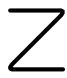
\includegraphics[keepaspectratio]{images/part001_11d71cd9.jpg}}

注. 1) 一个微分方程 (1) 在给定点处取同一值的积分可以有无穷多个。例如，数量微分方程 \(x' = 2\sqrt{|x|}\) 以由下列式子定义的诸函数

\[
\begin{array}{l l} u (t) = 0 & \text { for } \quad - \beta \leqslant t \leqslant \alpha \\ u (t) = - (t + \beta) ^ {2} & \text { for } \quad t \leqslant - \beta \\ u (t) = (t - \alpha) ^ {2} & \text { for } \quad t \geqslant \alpha \end{array}
\]

为其在点 t = 0 处取值 0 的积分，这里 \(\alpha\) 与 \(\beta\) 为任意正数。

\begin{enumerate}
\def\labelenumi{\arabic{enumi})}
\setcounter{enumi}{1}
\tightlist
\item
  当 \(\mathbf{E}\) 是任意无穷维的完备赋范空间时，佩亚诺定理不再成立（IV，第 204 页，习题 18）。
\end{enumerate}

\subsection{近似解的比较}

在下面，I 与 H 仍如前分别表示 R 中所包含的一个区间与赋范空间 E 中的一个开集；\(t_{0}\) 是 I 的一点。

定义 1. 给定定义在 I 上的正实函数 \(t \mapsto k(t)\)，称映射 \(\mathbf{f}\)（从 \(\mathrm{I} \times \mathrm{H}\) 到 E 中）关于函数 \(k(t)\) 是利普希茨的，如果对每个 \(\mathbf{x} \in \mathrm{H}\)，函数 \(t \mapsto \mathbf{f}(t, \mathbf{x})\) 在 I 上规则，并且对每个 \(t \in \mathrm{I}\) 与 H 中的每一对点 \(\mathbf{x}_1, \mathbf{x}_2\)，有（“利普希茨条件”）

\[
\left\| \mathbf {f} (t, \mathbf {x} _ {1}) - \mathbf {f} (t, \mathbf {x} _ {2}) \right\| \leqslant k (t) \left\| \mathbf {x} _ {1} - \mathbf {x} _ {2} \right\|.\tag{8}
\]

我们说 \(\mathbf{f}\) 在 \(\mathrm{I} \times \mathrm{H}\) 上（不加限定地说）是利普希茨的，如果它关于某个常数 \(k \geqslant 0\) 在该集合上是利普希茨的。显然，\(\mathrm{I} \times \mathrm{H}\) 上的利普希茨函数满足 IV 第 165 页引理 1 的假设（反之不真）；当 \(\mathbf{f}\) 在 \(\mathrm{I} \times \mathrm{H}\) 上是利普希茨的时，就称微分方程

\[
\mathbf {x} ^ {\prime} = \mathbf {f} (t, \mathbf {x})\tag{1}
\]

是利普希茨的（在 I × H 上）。

例. 当 E = R 且 H 是 R 中的一个区间时，若函数 \(f(t, x)\) 具有偏导数 \(f_{x}^{\prime}\)（II，第 74 页），在 I × H 的每一点 \((t, x)\) 处，且在 I × H 上 \(|f_{x}^{\prime}(t, x)| \leqslant k(t)\)，则由中值定理，条件 (8) 得到满足；我们以后将看到这个例子怎样推广到 E 为任意赋范空间的情形。

若 f 在 \(I \times H\) 上是利普希茨的，则对每个紧子区间 \(J \times S\) 与每个开球 \(J \subset I\)，f 在 \(S \subset H\) 上有界。于是可以应用命题 3（IV，第 166 页），它给出方程 (1) 的近似解的存在性。但我们还有下面的命题，它使我们可以比较两个近似解：

命题 5. 设 \(k(t)\) 是实规则函数且在 I 上 \(>0\)，并设 \(\mathbf{f}(t, \mathbf{x})\) 是已定义且关于 \(k(t)\) 在 \(\mathrm{I} \times \mathrm{H}\) 上为利普希茨的函数。若 \(\mathbf{u}\) 与 \(\mathbf{v}\) 是 (1) 的两个近似解，其精确度分别为 \(\varepsilon_1\) 与 \(\varepsilon_2\)，都定义在 I 上且取值于 H 中，则对每个 \(t \in \mathrm{I}\)（只要 \(t \geqslant t_0\)），

\[
\left\| \mathbf {u} (t) - \mathbf {v} (t) \right\| \leqslant \left\| \mathbf {u} \left(t _ {0}\right) - \mathbf {v} \left(t _ {0}\right) \right\| \Phi (t) + \left(\varepsilon_ {1} + \varepsilon_ {2}\right) \Psi (t)\tag{9}
\]

其中

\[
\left\{ \begin{array}{l} \Phi (t) = 1 + \int_ {t _ {0}} ^ {t} k (s) \exp \left(\int_ {s} ^ {t} k (\tau) d \tau\right) d s \\ \Psi (t) = t - t _ {0} + \int_ {t _ {0}} ^ {t} (s - t _ {0}) k (s) \exp \left(\int_ {s} ^ {t} k (\tau) d \tau\right) d s. \end{array} \right.\tag{10}
\]

由关系式 \(\left\| \mathbf{u}'(t) - \mathbf{f}(t, \mathbf{u}(t)) \right\| \leqslant \varepsilon_1\)（它在某个可数集的补集上成立），借助中值定理推出

\[
\left\| \mathbf {u} (t) - \mathbf {u} (t _ {0}) - \int_ {t _ {0}} ^ {t} \mathbf {f} (s, \mathbf {u} (s)) d s \right\| \leqslant \varepsilon_ {1} (t - t _ {0})
\]

同理可得

\[
\left\| \mathbf {v} (t) - \mathbf {v} (t _ {0}) - \int_ {t _ {0}} ^ {t} \mathbf {f} (s, \mathbf {v} (s)) d s \right\| \leqslant \varepsilon_ {2} (t - t _ {0})
\]

由此得

\[
\begin{array}{l} \| \mathbf {u} (t) - \mathbf {v} (t) \| \leqslant \| \mathbf {u} (t _ {0}) - \mathbf {v} (t _ {0}) \| \\ \qquad + \left\| \int_ {t _ {0}} ^ {t} (\mathbf {f} (s, \mathbf {u} (s)) - \mathbf {f} (s, \mathbf {v} (s))) d s \right\| + (\varepsilon_ {1} + \varepsilon_ {2}) (t - t _ {0}). \end{array}
\]

由利普希茨条件 (8) 有

\[
\begin{array}{r l} \left\| \int_ {t _ {0}} ^ {t} (\mathbf {f} (s, \mathbf {u} (s)) - \mathbf {f} (s, \mathbf {v} (s))) d s \right\| & \leqslant \int_ {t _ {0}} ^ {t} \| \mathbf {f} (s, \mathbf {u} (s)) - \mathbf {f} (s, \mathbf {v} (s)) \| d s \\ & \leqslant \int_ {t _ {0}} ^ {t} k (s) \| \mathbf {u} (s) - \mathbf {v} (s) \| d s \end{array}
\]

由此，令 \(w(t) = \|\mathbf{u}(t) - \mathbf{v}(t)\|\)，即得

\[
w (t) \leqslant w \left(t _ {0}\right) + \left(\varepsilon_ {1} + \varepsilon_ {2}\right) \left(t - t _ {0}\right) + \int_ {t _ {0}} ^ {t} k (s) w (s) d s.\tag{11}
\]

因此本命题是下述引理的推论：

引理 2. 若 \(w\) 是区间 \([t_0, t_1]\) 上的连续实函数且满足不等式

\[
w (t) \leqslant \varphi (t) + \int_ {t _ {0}} ^ {t} k (s) w (s) d s\tag{12}
\]

其中 \(\varphi\) 是规则函数 \(\geqslant 0\) 在 \([t_0, t_1]\) 上，则对 \(t_0 \leqslant t \leqslant t_1\)，

\[
w (t) \leqslant \varphi (t) + \int_ {t _ {0}} ^ {t} \varphi (s) k (s) \exp \left(\int_ {s} ^ {t} k (\tau) d \tau\right) d s.\tag{13}
\]

令 \(y(t) = \int_{t_0}^{t} k(s)w(s)ds\)；关系式 (12) 蕴含

\[
y ^ {\prime} (t) - k (t) y (t) \leqslant \varphi (t) k (t)\tag{14}
\]

在一个可数集的补集上。

令 \(z(t) = y(t)\exp \left(-\int_{t_0}^t k(s)ds\right)\)；则 (14) 等价于

\[
z ^ {\prime} (t) \leqslant \varphi (t) k (t) \exp \left(- \int_ {t _ {0}} ^ {t} k (s) d s\right).
\]

对此不等式应用中值定理（I，第 15 页，定理 2），并注意到 \(z(t_0) = 0\)，便得到

\[
z (t) \leqslant \int_ {t _ {0}} ^ {t} \varphi (s) k (s) \exp \left(- \int_ {t _ {0}} ^ {s} k (\tau) d \tau\right) d s
\]

由此得

\[
y (t) \leqslant \int_ {t _ {0}} ^ {t} \varphi (s) k (s) \exp \left(\int_ {s} ^ {t} k (\tau) d \tau\right) d s
\]

又因 \(w(t) \leqslant \varphi(t) + y(t)\)，这样就得到 (13)。

推论. 设 f 是关于常数 k \textgreater{} 0、定义在 I × H 上的利普希茨函数。若 u 与 v 是 (1) 的两个近似解，其精确度分别为 \(\varepsilon_{1}\) 与 \(\varepsilon_{2}\)，都定义在 I 上且取值于 H 中，则对一切 \(t \in I\)，

\[
\| \mathbf {u} (t) - \mathbf {v} (t) \| \leqslant \| \mathbf {u} (t _ {0}) - \mathbf {v} (t _ {0}) \| e ^ {k | t - t _ {0} |} + (\varepsilon_ {1} + \varepsilon_ {2}) \frac {e ^ {k | t - t _ {0} |} - 1}{k}.\tag{15}
\]

当 \(t \geqslant t_0\) 时，此不等式实际上是 (9) 的直接推论；要对 \(t \leqslant t_0\) 证明它，只需把它应用于方程

\[
{\frac {d \mathbf {x}}{d s}} = - \mathbf {f} (- s, \mathbf {x})
\]

它是通过变量代换 t = -s 从 (1) 得到的。

注. 1) 当 k = 0 时，不等式 (15) 换成不等式

\[
\left\| \mathbf {u} (t) - \mathbf {v} (t) \right\| \leqslant \left\| \mathbf {u} \left(t _ {0}\right) - \mathbf {v} \left(t _ {0}\right) \right\| + \left(\varepsilon_ {1} + \varepsilon_ {2}\right) | t - t _ {0} |
\]

其证明是直接的。

\begin{enumerate}
\def\labelenumi{\arabic{enumi})}
\setcounter{enumi}{1}
\tightlist
\item
  当 E 是有限维且 f 在 \(I \times H\) 上是利普希茨的时候，可以不用选择公理（IV，第 199 页，习题 1 b)）来证明 (1) 的近似解的存在性（IV，第 166 页，命题 3）。
\end{enumerate}

命题 6. 设 f 与 g 是定义在 I × H 上的两个函数，它们满足 IV 第 165 页引理 1 的假设，并且在 I × H 上

\[
\left\| \mathbf {f} (t, \mathbf {x}) - \mathbf {g} (t, \mathbf {x}) \right\| \leqslant \alpha .\tag{16}
\]

再设 \(\mathbf{g}\) 是关于常数 \(k > 0\) 在 \(\mathrm{I} \times \mathrm{H}\) 上为利普希茨的函数。在这些条件下，若 \(\mathbf{u}\) 是 \(\mathbf{x}' = \mathbf{f}(t, \mathbf{x})\) 的精确到 \(\varepsilon_1\) 的近似解，它定义在 \(\mathrm{I}\) 上、取值于 \(\mathrm{H}\) 中，而 \(\mathbf{v}\) 是 \(\mathbf{x}' = \mathbf{g}(t, \mathbf{x})\) 的精确到 \(\varepsilon_2\) 的近似解，它定义在 \(\mathrm{I}\) 上、取值于 \(\mathrm{H}\) 中，则对一切 \(t \in \mathrm{I}\)

\[
\| \mathbf {u} (t) - \mathbf {v} (t) \| \leqslant \| \mathbf {u} (t _ {0}) - \mathbf {v} (t _ {0}) \| e ^ {k | t - t _ {0} |} + (\alpha + \varepsilon_ {1} + \varepsilon_ {2}) \frac {e ^ {k | t - t _ {0} |} - 1}{k}.\tag{17}
\]

的确

\[
\left| \left| \mathbf {u} ^ {\prime} (t) - \mathbf {g} (t, \mathbf {u} (t)) \right| \right| \leqslant \alpha + \varepsilon_ {1}
\]

此式对 I 中某个可数子集在 I 中的补集的所有 t 成立；换言之，u 是 \(\mathbf{x}^{\prime} = \mathbf{g}(t, \mathbf{x})\) 的精确到 \(\alpha + \varepsilon_{1}\) 的近似解，于是应用 IV 第 169 页的命题 5 即得不等式 (17)。

\subsection{利普希茨方程与局部利普希茨方程的解的存在性与唯一性}

定理 1（柯西）. 设 \(\mathbf{f}\) 是 \(\mathrm{I} \times \mathrm{H}\) 上的利普希茨函数，设 \(\mathrm{J}\) 是 \(\mathrm{I}\) 的一个不退化为一点的紧子区间，\(t_0\) 是 \(\mathrm{J}\) 的一点，\(\mathrm{S}\) 是以 \(\mathbf{x}_0\) 为中心、以 \(r\) 为半径、包含于 \(\mathrm{H}\) 中的开球，而 \(\mathrm{M}\) 是 \(\| \mathbf{f}(t, \mathbf{x})\|\) 在 \(\mathrm{J} \times \mathrm{S}\) 上的上确界。在这些条件下，对每个紧区间 \(\mathrm{K}\)，若它不退化为一点、包含于 \(\mathrm{J}\) 与 \(]t_0 - r / M\)、\(t_0 + r / M[\) 的交中且包含 \(t_0\)，则存在微分方程 \(\mathbf{x}' = \mathbf{f}(t, \mathbf{x})\) 的唯一一个解，它定义在 \(\mathrm{K}\) 上、取值于 \(\mathrm{S}\) 中、且在点 \(\mathbf{x}_0\) 处等于 \(t_0\) 。

的确，当 \(\varepsilon > 0\) 足够小时，\(F_{\varepsilon}\)（即 (1) 的精确到 \(\varepsilon\) 、定义在 K 上、取值于 S 中且等于 \(x_{0}\) 于点 \(t_{0}\) 的近似解）非空（IV，第 166 页，命题 3）；此外，若 u 与 v 都属于 \(F_{\varepsilon}\) ，则由 (15)（IV，第 170 页）

\[
\| \mathbf {u} (t) - \mathbf {v} (t) \| \leqslant 2 \varepsilon \frac {e ^ {k | t - t _ {0} |} - 1}{k}
\]

对一切 \(t \in K\) ，于是诸集 \(F_{\varepsilon}\) 构成一个滤基 G，它在 K 上一致收敛于一个连续函数 w，后者等于 \(x_{0}\) 于 \(t_{0}\) ；而且 w 取值于 S 中，因为当 \(\varepsilon\) 足够小时，诸函数 \(u \in F_{\varepsilon}\) 的值都属于一个包含于 S 中的闭球。由于 \(\mathbf{f}(t, \mathbf{u}(t))\) 沿 G 在 K 上一致趋于 \(\mathbf{f}(t, \mathbf{w}(t))\) ，w 满足 IV 第 165 页的方程 (6)，因而是 (1) 的解。解的唯一性由 IV 第 170 页的不等式 (15) 立即得出，其中取 \(\varepsilon_{1} = \varepsilon_{2} = 0\) 与 \(\mathbf{u}(t_{0}) = \mathbf{v}(t_{0})\) 。

我们说函数 \(\mathbf{f}\)（定义在 \(\mathrm{I} \times \mathrm{H}\) 上）是局部利普希茨的，如果对 \((t, \mathbf{x})\) 的每个点 \(\mathrm{I} \times \mathrm{H}\) ，存在 \(\mathrm{V}\) 的一个邻域 \(t\)（关于 \(\mathrm{I}\) ）与 \(\mathrm{S}\) 的一个邻域 \(\mathbf{x}\)，使得 \(\mathbf{f}\) 在 \(\mathrm{V} \times \mathrm{S}\) 上是利普希茨的（常数 \(k\) 依赖于 \(\mathrm{V}\) 与 \(\mathrm{S}\) ）。由博雷尔–勒贝格定理，对每个紧区间 \(\mathrm{J} \subset \mathrm{I}\) 与每个点 \(\mathbf{x}_0 \in \mathrm{H}\)，存在以 \(\mathrm{S}\) 为中心、包含于 \(\mathbf{x}_0\) 中的开球 \(\mathrm{H}\)，使得 \(\mathbf{f}\) 在 \(\mathrm{J} \times \mathrm{S}\) 上是利普希茨的；于是 \(\mathbf{f}\) 满足 IV 第 3 页引理 1 的假设。当 \(\mathbf{f}\) 在 \(\mathrm{I} \times \mathrm{H}\) 上是局部利普希茨的时候，我们称方程 \(\mathbf{x}' = \mathbf{f}(t, \mathbf{x})\) 在 \(\mathrm{I} \times \mathrm{H}\) 上是局部利普希茨的。

我们要对局部利普希茨方程推广并阐明 IV 第 10 页的定理 1；我们限于 \(t_0\) 是区间 I 的左端点的情形；对 \(t_0\) 是 I 的任意点的情形，容易化归为上述情形（参看 IV，§ IV ??，第 9 页，推论）。

定理 2. 设 \(\mathbf{I} \subset \mathbf{R}\) 是一个（不退化为一点的）区间，其左端点为 \(t_0 \in \mathbf{I}\) ；设 \(\mathbf{H}\) 是 \(\mathbf{E}\) 中的一个非空开集，并设 \(\mathbf{f}\) 是 \(\mathbf{I} \times \mathbf{H}\) 上的局部利普希茨函数。

\(1^{\circ}\) 对 \(\mathbf{x}_0\in \mathrm{H}\) ，存在最大的区间 \(\mathbf{J}\subset \mathbf{I}\)（其左端点为 \(t_0\in \mathbf{J}\) ），在该区间上存在一个积分 \(\mathbf{u}\) ，即方程 \(\mathbf{x}' = \mathbf{f}(t,\mathbf{x})\) 的、取值于 H 中且等于 \(\mathbf{x}_0\) 于点 \(t_0\) 的积分；这个积分是唯一的。

\(2^{\circ}\) 若 \(\mathrm{J} \neq \mathrm{I}\) ，则 \(\mathrm{J}\) 是长度有限的半开区间 \([t_0, \beta[\) ；此外，对每个紧子集 \(\mathbf{K} \subset \mathbf{H}\) ，集合 \(\overline{\mathbf{u}}^{-1}(\mathbf{K})\) 是 \(\mathbf{R}\) 的紧子集。

\(3^{\circ}\) 若 \(\mathbf{J}\) 有界，且若 \(\mathbf{f}(t,\mathbf{u}(t))\) 在 \(\mathbf{J}\) 上有界，则 \(\mathbf{u}(t)\) 在 \(\mathbf{c}\) 的右端点处有左极限 \(\mathbf{J}\) ；此外，若 \(\mathbf{J} \neq \mathbf{I}\) ，则 \(\mathbf{c}\) 是 \(\mathbf{H}\) 在 \(\mathbf{E}\) 中的边界点。

\(1^{\circ}\) 设 \(\mathfrak{M}\) 是由这样的区间 L（不退化为一点、左端点为 \(t_0 \in L\) 、包含于 I）组成的集合：在 L 上存在 (1)（IV，第 163 页）的、取值于 H 中且等于 \(\mathbf{x}_0\) 于 \(t_0\) 的解；由定理 1（IV，第 171 页），集合 \(\mathfrak{M}\) 非空。设 L 与 L' 是属于 \(\mathfrak{M}\) 的两个区间，例如设 L \(\subset\) L'；若 u 与 v 是 (1) 的两个积分，分别定义在 L 与 L' 上、取值于 H 中且等于 \(\mathbf{x}_0\) 于 \(t_0\) ，我们将看到 v 是 u 的扩张。的确，设 \(t_1\) 是使 \(t \in L\) 满足 \(\mathbf{u}(s) = \mathbf{v}(s)\) （对 \(t_0 \leqslant s \leqslant t\) ）的 t 组成的集合的上确界；我们将证明 \(t_1\) 是 L 的右端点。若非如此，则由连续性有 \(\mathbf{u}(t_1) = \mathbf{v}(t_1)\) ，且 \(\mathbf{x}_1 = \mathbf{u}(t_1)\) 属于 H；由于 f 是局部利普希茨的，定理 1 表明只能存在 (1) 的一个在 \(t_1\) 的邻域上定义、取值于 H 中且等于 \(\mathbf{x}_1\) 于 \(t_1\) 的积分；因此假定 \(t_1\) 不是 L 的右端点便导致矛盾。现在我们看到，若 J 是诸区间 L \(\in\) M 的并，则存在 (1) 的唯一一个积分 u，它定义在 J 上、取值于 H 中且等于 \(\mathbf{x}_0\) 于 \(t_0\) 。

\(2^{\circ}\) 设 \(\mathrm{J} \neq \mathrm{I}\) ，并设 \(\beta\) 是 \(\mathrm{J}\) 的右端点；若 \(\beta\) 是 \(\mathrm{I}\) 的右端点，则 \(\beta \in \mathrm{I}\) （于是 \(\beta\) 是有限的），且由假设 \(\mathrm{J} = [t_0, \beta[\) 。今设 \(\beta\) 不是 \(\mathrm{I}\) 的右端点；若 \(\beta \in \mathrm{J}\) ，则 \(\mathbf{u}(\beta) = \mathbf{c}\) 属于 \(\mathrm{H}\) ；由定理 1，存在 (1) 的一个取值于 \(\mathrm{H}\) 中、定义在一个区间上的积分

\[
[ \beta , \beta_ {1} [ \subset I
\]

且等于 \(\mathbf{c}\) 于 \(\beta\) ；这样 \(\mathrm{J}\) 就不是 \(\mathfrak{M}\) 中最大的区间，这是荒谬的；故 \(\mathrm{J} = [t_0, \beta[\) 。

若 K 是 H 的紧子集，则 \(\overline{\mathbf{u}}^{-1}(\mathbf{K})\) 在 J 中是闭的；我们将看到存在 \(\gamma\in J\) 使得 \(\overline{\mathbf{u}}^{-1}(\mathbf{K})\) 包含于 \([t_{0},\gamma]\) 中，这就证明 \(\overline{\mathbf{u}}^{-1}(\mathbf{K})\) 是紧的。若不然，就会存在一点 \(c\in K\) 使得 \((\beta,\mathbf{c})\) 是点 \((t,\mathbf{u}(t))\)（其中 \(t<\beta\) 与 \(\mathbf{u}(t)\in\mathbf{K}\) ）所成之集的聚点。由于 \(\beta\in I\) 与 \(c\in H\) ，则存在 \(\beta\) 在 I 中的邻域 V，以及以 c 为中心、半径 r 且包含于 H 中的开球 S，使得 f 在 V×S 上是利普希茨的且有界；令 M 为 \(\|\mathbf{f}(t,\mathbf{x})\|\) 在该集合上的上确界。由假设存在 \(t_{1}\in J\) 使得 \(\beta-t_{1}<r/2M\) 、\(t_{1}\in V\) 与 \(\|\mathbf{u}(t_{1})-\mathbf{c}\|\leqslant r/2\) ；定理 1 表明存在 (1) 的唯一一个积分，它取值于 H 中、定义在包含 \([t_{1},t_{2}]\) 的区间 \(\beta\) 上、且等于 \(\mathbf{u}(t_{1})\) 于 \(t_{1}\) ；由于这个区间在区间 \([t_{1},\beta[\) 上与 u 一致，便推出 \(J=[t_{0},\beta[\) 不是 M 中最大的区间，这是荒谬的。

\(3^{\circ}\) 设 \(\mathbf{J}\) 有界且 \(\| \mathbf{f}(t,\mathbf{u}(t))\| \leqslant M\) 在 \(\mathbf{J}\) 上成立；则在 \(\| \mathbf{u}'(t)\| \leqslant \mathbf{M}\) 于 \(\mathbf{J}\) 的一个可数子集的补集上成立；于是由中值定理，对 \(\| \mathbf{u}(s) - \mathbf{u}(t)\| \leqslant \mathbf{M} |s - t|\) 与 \(s\)（都属于 \(t\) ）有 \(\mathbf{J}\) ；由柯西准则，\(\mathbf{u}\) 有左极限 \(\mathbf{c}\) 于 \(\beta\) 处（它是 \(\mathbf{J}\) 的右端点）；若 \(\mathbf{J} \neq \mathbf{I}\) ，则 \(\mathbf{c}\) 不可能属于 \(\mathbf{H}\) ，因为把 \(\mathbf{u}\) 在 \(\beta\) 处连续延拓后，\(\mathbf{u}\) 就成为 (1) 的一个取值于 \(\mathbf{H}\) 中、定义在区间 \([t_0, \beta]\) 上且等于 \(\mathbf{x}_0\) 于 \(t_0\) 的积分；于是就有 \(\mathbf{J} = [t_0, \beta]\) ，这与我们在 \(2^{\circ}\) 中已看到的相矛盾。

推论 1. 若 H = E 且 J ≠ I，则 \(\mathbf{f}(t, \mathbf{u}(t))\) 在 J 上不是有界的；进而，若 E 是有限维的，则 \(\| \mathbf{u}(t) \|\) 在 J 的右端点处有左极限 \(+\infty\) 。

第一部分是定理 2 第三部分的直接推论。若 E 是有限维的，则每个闭球 \(S \subset E\) 是紧的，于是定理 2 的第二部分表明存在 \(\gamma \in J\) 使得 \(\mathbf{u}(t) \notin \mathbf{S}\) 对 \(t > \gamma\) 成立。

若 E 是有限维的，可能发生这样的情况：\(J \neq I\) 而 \(\|\mathbf{u}(t)\|\) 当 t 趋于 J 的右端点时保持有界（IV，第 200 页，习题 5）。

推论 2. 若在 I × H 上函数 f 关于一个规则函数 k(t) 是利普希茨的，且若 J 的右端点 β 属于 I，则 u 在 β 处有左极限；若 H = E 且 f 在 I × E 上关于一个规则函数 k(t) 是利普希茨的，则 J = I。

的确，若 \(\beta \in \mathbf{I}\) ，则存在 \(\mathrm{V}\) 在 \(\beta\) 中的一个紧邻域 \(\mathbf{I}\) ，使得 \(\mathbf{f}(t, \mathbf{x}_0)\) 与 \(k(t)\) 在 \(\mathrm{V}\) 上有界；于是 \(\| \mathbf{f}(t, \mathbf{x}) \| \leqslant m \| x \| + h\) （\(m\) 与 \(h\) 为常数）

在 \(V \times H\) 上成立，由此 \(\left\|\mathbf{u}^{\prime}(t)\right\| \leqslant m \left\|\mathbf{u}(t)\right\| + h\) 在 \(V \cap J\) 的一个可数子集的补集上成立，从而 \(\left\|\mathbf{u}(t)\right\| \leqslant m \int_{t_{0}}^{t} \left\|\mathbf{u}(s)\right\| ds + q\) （q 为常数）在 \(V \cap J\) 上成立；引理 2（IV，第 170 页）表明 \(\left\|\mathbf{u}(t)\right\| \leqslant c e^{mt} + d\) （c 与 d 为常数）在 \(V \cap J\) 上成立，于是 \(\mathbf{f}(t, \mathbf{u}(t))\) 在 J 上保持有界，从而由 IV 第 172 页的定理 2 即得本推论。

例. 1) 对形如 \(\mathbf{x}' = \mathbf{g}(t)\) 的微分方程（其中 \(\mathbf{g}\) 在 I 上是规则的），每个积分 \(\mathbf{u}\) 显然都定义在整个 I 上。应当注意，\(\mathbf{u}\) 可以在 I 上有界而 \(\mathbf{g}(t)\) 并不如此。

\begin{enumerate}
\def\labelenumi{\arabic{enumi})}
\setcounter{enumi}{1}
\item
  对数量方程 \(x' = \sqrt{1 - x^2}\) 有 \(I = R\) ，\(H = ] - 1, +1[\) 。若取 \(t_0 = x_0 = 0\) ，则相应的积分是 \(\sin t\) ，其定义区间是包含 0 且使 \(\sin t\) 的导数为正的最大区间，也就是说，\(] - \pi / 2, +\pi / 2[\) ；在这个区间的端点处，积分趋于 \(H\) 的一个端点。
\item
  对数量方程 \(x' = 1 + x^{2}\) 有 I = H = R；在 t = 0 处为零的积分是 \(\tan t\) ，而包含 0 且使该函数连续的最大区间是 \(J = ] - \pi/2, +\pi/2[\) ；且 \(|\tan t|\) 在 J 的端点处趋于 \(+\infty\) （参看 IV，第 173 页，推论 1）。
\item
  对数量方程 \(x' = \sin tx\) 有 I = H = R，且右端在 I × H 上有界，故（IV，第 173 页，推论 1）每个积分都定义在整个 R 上。
\end{enumerate}

\subsection{积分作为参数函数的连续性}

命题 6（IV，第 171 页）表明：当一个微分方程

\[
\mathbf {x} ^ {\prime} = \mathbf {f} (t, \mathbf {x})
\]

“接近”于一个利普希茨方程 \(\mathbf{x}^{\prime} = \mathbf{g}(t, \mathbf{x})\) ，且当假定两个方程在同一区间上都有近似解时，这两个近似解是“接近”的；我们将阐明这个结果，办法是证明：只要利普希茨方程 \(\mathbf{x}^{\prime} = \mathbf{g}(t, \mathbf{x})\) 在某区间上存在解，便蕴含方程 \(\mathbf{x}^{\prime} = \mathbf{f}(t, \mathbf{x})\) 在同一区间上近似解的存在，前提是在该区间上，方程 \(\mathbf{x}^{\prime} = \mathbf{g}(t, \mathbf{x})\) 的解的值并不“太接近” H 的边界。

命题 7. 设 f 与 g 是定义在 I × H 上的两个函数，满足 IV 第 165 页引理 1 的假设，并且在 I × H 上

\[
\left\| \mathbf {f} (t, \mathbf {x}) - \mathbf {g} (t, \mathbf {x}) \right\| \leqslant \alpha .\tag{16}
\]

再设 \(\mathbf{g}\) 关于常数 \(k > 0\) 在 \(\mathrm{I} \times \mathrm{H}\) 上是利普希茨的，且 \(\mathbf{f}\) 在 \(\mathrm{I} \times \mathrm{H}\) 上是局部利普希茨的，或者 \(\mathrm{E}\) 是有限维的。设 \((t_0, \mathbf{x}_0)\) 是 \(\mathrm{I} \times \mathrm{H}\) 的一点，\(\mu\) 是一个数 \(>0\) ，并设

\[
\varphi (t) = \mu e ^ {k (t - t _ {0})} + \alpha \frac {e ^ {k (t - t _ {0})} - 1}{k}.
\]

设 \(\mathbf{u}\) 是方程 \(\mathbf{x}' = \mathbf{g}(t, \mathbf{x})\) 的一个积分，它定义在包含于 I 的区间 \(\mathrm{K} = [t_0, b[\) 上、等于 \(\mathbf{x}_0\) 于点 \(t_0\) ，并且对一切 \(t \in \mathrm{K}\) ，以 \(\mathbf{u}(t)\) 为中心、以 \(\varphi(t)\) 为半径的闭球都包含于 H 中。在这些条件下，对每个满足 \(\mathbf{y} \in \mathrm{H}\) 的 \(\| \mathbf{y} - \mathbf{x}_0 \| \leqslant \mu\) ，便存在 \(\mathbf{v}\) ，它是方程 \(\mathbf{x}' = \mathbf{f}(t, \mathbf{x})\) 的一个积分，定义在 K 上、取值于 H 中且等于 \(\mathbf{y}\) 于点 \(t_0\) ；此外，在 K 上有 \(\| \mathbf{u}(t) - \mathbf{v}(t) \| \leqslant \varphi(t)\) 。

设 M 是 \(\mathbf{x}^{\prime} = \mathbf{f}(t, \mathbf{x})\) 的积分所成的族，其中每个积分都取值于 H 中、在 \(t_{0}\) 处等于 y、且定义在一个包含于 I 的半开区间 \([t_{0}, \tau[\) 上（该区间随所考虑的积分而异）。由 IV 第 171 页的定理 1（当 f 是局部利普希茨时）或 IV 第 167 页的推论（当 E 是有限维时），M 非空，且与 IV 第 166 页命题 3 中同样的推理表明，M 依序关系“v 是 w 的限制”是归纳的。设 \(v_{0}\) 是 M 的一个极大元，\([t_{0}, t_{1}[\) 是 \(v_{0}\) 的定义区间；由 IV 第 171 页的命题 6，一切都归结为证明 \(t_{1} \geqslant b\) 。若不然，则有

\[
\left\| \mathbf {u} (t) - \mathbf {v} _ {0} (t) \right\| \leqslant \varphi (t)
\]

在区间 \([t_0, t_1[\) 上此式由命题 6 得出；而在紧区间 \([t_0, t_1]\) 上，规则函数 \(\mathbf{g}(t, \mathbf{u}(t))\) 有界，故函数 \(\mathbf{g}(t, \mathbf{v}_0(t))\) 在区间 \([t_0, t_1[\) 上有界，因为在此区间上 \(\| \mathbf{g}(t, \mathbf{v}_0(t)) \| \leqslant \| \mathbf{g}(t, \mathbf{u}(t)) \| + k\varphi(t)\) 。由于 \(\mathbf{v}_0\) 是 \(\mathbf{x}' = \mathbf{g}(t, \mathbf{x})\) 的精确到 \(\alpha\) 的近似解（在 \([t_0, t_1[\) 上），故存在数 \(M > 0\) 使得在此区间上除去一个可数集的点以外有 \(\| \mathbf{v}_0'(t) \| \leqslant M\) ；于是中值定理表明 \(\| \mathbf{v}_0(s) - \mathbf{v}_0(t) \| \leqslant M |s - t|\) ，对每对点 \(s\) 与 \(t\)（都属于 \([t_0, t_1[\) ）成立，从而（由柯西准则）\(\mathbf{v}_0(t)\) 有左极限 \(\mathbf{c}\) 于点 \(t_1\) ，并且由连续性有 \(\| \mathbf{c} - \mathbf{u}(t_1) \| \leqslant \varphi(t_1)\) ，故 \(\mathbf{c} \in H\) 。于是由 IV 第 171 页定理 1 或 IV 第 167 页推论可见，存在 \(\mathbf{x}' = \mathbf{f}(t, \mathbf{x})\) 的一个积分，它定义在区间 \([t_1, t_2[\) 上且等于 \(\mathbf{c}\) 于 \(t_1\) ，这与 \(\mathbf{v}_0\) 的定义相矛盾。

定理 3. 设 F 是一个拓扑空间，f 是从 I × H × F 到 E 中的一个映射，使得对每个 \(\xi \in F\) ，函数 \((t, \mathbf{x}) \mapsto \mathbf{f}(t, \mathbf{x}, \xi)\) 在 I × H 上是利普希茨的，并且当 \(\xi\) 趋于 \(\xi_{0}\) 时，\(\mathbf{f}(t, \mathbf{x}, \xi)\) 在 I × H 上一致趋于 \(\mathbf{f}(t, \mathbf{x}, \xi_{0})\) 。设 \(\mathbf{u}_{0}(t)\) 是 \(\mathbf{x}' = \mathbf{f}(t, \mathbf{x}, \xi_{0})\) 的一个积分，它定义在包含于 I 中的区间 J = {[}t₀, b{[} 上、取值于 H 中且在 t₀ 处等于 \(x_{0}\) 。对每个包含于 J 中的紧区间 {[}t₀, t₁{]} ，存在 \(\xi_{0}\) 在 F 中的一个邻域 V，使得对每个 \(\xi \in V\) ，方程 \(\mathbf{x}' = \mathbf{f}(t, \mathbf{x}, \xi)\) 有一个（且仅有一个）积分 \(\mathbf{u}(t, \xi)\) ，它定义在 {[}t₀, t₁{]} 上、取值于 H 中且在 t₀ 处等于 \(x_{0}\) ；而且，当 \(\xi\) 趋于 \(\xi_{0}\) 时，解 \(\mathbf{u}(t, \xi)\) 在 \(\mathbf{u}_{0}(t)\)[{t₀, t₁}]{ 上一致趋于 } 。

的确，取 r \textgreater{} 0，使得对 \(t_{0} \leqslant t \leqslant t_{1}\) ，以 \(\mathbf{u}_{0}(t)\) 为中心、以 r 为半径的闭球包含于 H 中；若 \(\mathbf{f}(t, \mathbf{x}, \xi)\) 关于常数 k \textgreater{} 0 在 I × H 上是利普希茨的，则取 \(\alpha\) 足够小，使 \(\alpha \frac{e^{k(t_{1}-t_{0})} - 1}{k} < r\) ；取 V 使得对每个 \(\xi \in V\) ，在 I × H 上有 \(\|f(t, \mathbf{x}, \xi) - f(t, \mathbf{x}, \xi_{0})\| \leqslant \alpha\) ，就可以应用 IV 第 174 页的命题 7；此外，

\[
\| \mathbf {u} (t, \xi) - \mathbf {u} _ {0} (t) \| \leqslant \alpha \frac {e ^ {k \left(t _ {1} - t _ {0}\right)} - 1}{k}
\]

在 \([t_{0}, t_{1}]\) 上，这就完成了定理的证明。

注. 当 H = E 且 IV 第 174 页的条件 (16) 在 I × E 上满足时，IV 第 174 页的命题 7 可应用于 \(\mathbf{x}' = \mathbf{g}(t, \mathbf{x})\) 的每个解 u，在其有定义的任何区间上；甚至还可以假定 \(\mathbf{g}(t,\mathbf{x})\) 关于一个规则函数 \(k(t)\) 是利普希茨的，尽管该函数在此区间上未必有界。

\subsection{对初始条件的依赖性}

设 \(\mathbf{x}^{\prime}=\mathbf{f}(t,\mathbf{x})\) 是 \(I\times H\) 上的局部利普希茨方程；由定理 2（IV，第 172 页），对 \((t_{0},\mathbf{x}_{0})\) 的每个点 \(I\times H\) ，存在最大的区间 \(J(t_{0},\mathbf{x}_{0})\subset I\) （不退化为一点、包含 \(t_{0}\) ），在该区间上存在此方程的一个（且仅有的一个）积分，它等于 \(x_{0}\) 于 \(t_{0}\) ；我们将阐明这个积分以及其定义区间 \(J(t_{0},\mathbf{x}_{0})\) 依赖点 \((t_{0},\mathbf{x}_{0})\) 的方式。

定理 4. 设 \(\mathbf{f}\) 是 \(\mathrm{I} \times \mathrm{H}\) 上的局部利普希茨函数，而 \((a, \mathbf{b})\) 是 \(\mathrm{I} \times \mathrm{H}\) 的任意一点。

\(1^{\circ}\) 存在一个区间 \(\mathbf{K} \subset \mathbf{I}\) （即 \(a\) 在 \(\mathbf{I}\) 中的邻域）和一个 \(\mathbf{V}\) 在 \(\mathbf{b}\) 中的邻域 \(\mathbf{H}\) ，使得对 \((t_0, \mathbf{x}_0)\) 的每个点 \(\mathbf{K} \times \mathbf{V}\) ，存在一个（且仅有一个）积分 \(\mathbf{u}(t, t_0, \mathbf{x}_0)\) ，它定义在 \(\mathbf{K}\) 上、取值于 \(\mathbf{H}\) 中且等于 \(\mathbf{x}_0\) 于点 \(t_0\) （换言之，\(J(t_0, \mathbf{x}_0) \supset \mathbf{K}\) 对一切 \((t_0, \mathbf{x}_0) \in \mathbf{K} \times \mathbf{V}\) 成立）。

\(2^{\circ}\) 映射 \((t,t_0,\mathbf{x}_0)\mapsto \mathbf{u}(t,t_0,\mathbf{x}_0)\)（从 \(\mathrm{K}\times \mathrm{K}\times \mathrm{V}\) 到 H 中）是一致连续的。

\(3^{\circ}\) 存在 \(\mathbf{W} \subset \mathbf{V}\) 在 \(\mathbf{b}\) 中的一个邻域 \(\mathbf{H}\) ，使得对每个点

\[
(t, t _ {0}, \mathbf {x} _ {0}) \in \mathrm{K} \times \mathrm{K} \times \mathrm{W},
\]

方程 \(\mathbf{x}_{0} = \mathbf{u}(t_{0}, t, \mathbf{x})\) 在 V 上有唯一的解 x，它等于 \(\mathbf{u}(t, t_{0}, \mathbf{x}_{0})\)（“把积分关于积分常数解出”）。

\(1^{\circ}\) 设 S 是以 \(\mathbf{b}\) 为中心、以 \(r\) 为半径且包含于 H 中的球，并设 \(\mathrm{J}_0\) 是包含于 I 的区间，即 \(a\) 在 I 中的邻域，使得 \(\mathbf{f}\) 有界且是利普希茨的（关于某个常数 \(k\) ）于 \(\mathrm{J}_0 \times \mathrm{S}\) 上；用 M 表示 \(\| \mathbf{f}(t, \mathbf{x})\|\) 在 \(\mathrm{J}_0 \times \mathrm{S}\) 上的上确界。于是存在（IV，第 171 页，定理 1）一个区间 \(\mathrm{J} \subset \mathrm{J}_0\) （即 \(a\) 在 I 中的邻域）和一个积分 \(\mathbf{v}\) ，即方程 \(\mathbf{x}' = \mathbf{f}(t, \mathbf{x})\) 的一个积分，它定义在 J 上、取值于 S 中且等于 \(\mathbf{b}\) 于 \(a\) 。我们将看到，以 \(\mathbf{b}\) 为中心、以 \(r/2\) 为半径的开球 V，以及 J 与区间 \([a - l, a + l[\) （其中 \(l\) 足够小）的交 K，都合乎要求。的确，IV 第 174 页的命题 7（应用于集合 \(\mathrm{J}_0 \times \mathrm{S}\) 和 \(\alpha = 0\) 的情形）表明存在 \(\mathbf{x}' = \mathbf{f}(t, \mathbf{x})\) 的一个积分，它定义在 K 上、取值于 S 中且等于 \(\mathbf{x}_0\) 于一点 \(t_0 \in \mathrm{K}\) ，其条件是

\[
\left\| \mathbf {v} (t) - \mathbf {b} \right\| + \left\| \mathbf {v} (t _ {0}) - \mathbf {x} _ {0} \right\| e ^ {k | t - t _ {0} |} <   r\tag{18}
\]

对每个 \(t \in \mathbf{K}\) 。于是由中值定理有

\[
\| \mathbf {v} (t) - \mathbf {b} \| \leqslant \mathrm{M} | t - a | \leqslant \mathrm{M} l
\]

对每个 \(t \in \mathbf{K}\) ；由于 \(\| \mathbf{x}_0 - \mathbf{b} \| < r / 2\) ，可见只需取 \(l\) 使得

\[
\mathbf {M} l + (\mathbf {M} l + r / 2) e ^ {2 k l} <   r\tag{19}
\]

便可使关系式 (18) 对每个 \((t, t_{0}, \mathbf{x}_{0})\)（属于 \(K \times K \times V\) ）都成立。

\(2^{\circ}\) 由中值定理有

\[
\left\| \mathbf {u} (t _ {1}, t _ {0}, \mathbf {x} _ {0}) - \mathbf {u} (t _ {2}, t _ {0}, \mathbf {x} _ {0}) \right\| \leqslant \mathrm{M} \left| t _ {2} - t _ {1} \right|\tag{20}
\]

对 K 中的一切 \(t_0, t_1, t_2\) 与 V 中的 \(\mathbf{x}_0\) 。现在命题 5（IV，第 169 页）表明

\[
\left\| \mathbf {u} (t, t _ {0}, \mathbf {x} _ {1}) - \mathbf {u} (t, t _ {0}, \mathbf {x} _ {2}) \right\| \leqslant e ^ {2 k t} \left\| \mathbf {x} _ {2} - \mathbf {x} _ {1} \right\|\tag{21}
\]

对 K 中的每个 t 和 \(t_{0}\)，以及 V 中的 \(x_{1}\) 与 \(x_{2}\)。最后，若 \(t_{1}\) 与 \(t_{2}\) 是 K 中任意两点，

\[
\left\| \mathbf {u} \left(t _ {1}, t _ {2}, \mathbf {x} _ {0}\right) - \mathbf {u} \left(t _ {2}, t _ {2}, \mathbf {x} _ {0}\right) \right\| \leqslant \mathrm{M} \left| t _ {2} - t _ {1} \right|
\]

这是由中值定理得到的，也就是说

\[
\left\| \mathbf {u} (t _ {1}, t _ {2}, \mathbf {x} _ {0}) - \mathbf {x} _ {0} \right\| \leqslant \mathbf {M} \left| t _ {2} - t _ {1} \right|;
\]

由于 \(\mathbf{u}(t, t_2, \mathbf{x}_0)\) 与取值 \(\mathbf{u}(t_1, t_2, \mathbf{x}_0)\) 于点 \(t_1\) 的积分相同，命题 5（IV，第 169 页）表明

\[
\left\| \mathbf {u} (t, t _ {1}, \mathbf {x} _ {0}) - \mathbf {u} (t, t _ {2}, \mathbf {x} _ {0}) \right\| \leqslant \mathrm{Me} ^ {2 k l} | t _ {2} - t _ {1} |\tag{22}
\]

对 \(t, t_{1}, t_{2}\) 中的一切 \(\mathbf{K}\) 与 \(\mathbf{x}_{0}\) 中的一切 \(\mathrm{V}\) 都成立。于是三个不等式 (20)、(21) 与 (22) 证明了映射 \((t, t_{0}, \mathbf{x}_{0}) \mapsto \mathbf{u}(t, t_{0}, \mathbf{x}_{0})\) 在 \(\mathrm{K} \times \mathrm{K} \times \mathrm{V}\) 上的一致连续性。

\(3^{\circ}\) 由 (20)，有 \(\|\mathbf{u}(t, t_{0}, \mathbf{x}_{0}) - \mathbf{x}_{0}\| \leqslant \mathbf{M} |t - t_{0}| \leqslant 2\mathbf{M}l\) 于

\[
\mathbf {K} \times \mathbf {K} \times \mathbf {V}.
\]

若把 \(l\) 取得足够小，使 \(2\mathrm{M}l < r / 4\) ，则可以看出：若 \(\mathbf{x}_0\) 是以 \(\mathbf{W}\) 为中心、以 \(\mathbf{b}\) 为半径的开球 \(r / 4\) 中的任意一点，那么 \(\mathbf{u}(t,t_0,\mathbf{x}_0)\in \mathbf{V}\) 对任何 \(t\) 与 \(t_0\)（都属于 \(\mathbf{K}\) ）成立。若 \(\mathbf{x} = \mathbf{u}(t,t_0,\mathbf{x}_0)\) ，则函数 \(s\mapsto \mathbf{u}(s,t,\mathbf{x})\) 便定义在 \(\mathbf{K}\) 上，并且等于 (1) 的取值 \(\mathbf{x}\) 于点 \(t\) 的那个积分，也就是等于 \(\mathbf{u}(s,t_0,\mathbf{x}_0)\) ；特别地

\[
\mathbf {x} _ {0} = \mathbf {u} (t _ {0}, t _ {0}, \mathbf {x} _ {0}) = \mathbf {u} (t _ {0}, t, \mathbf {x}).
\]

此外，若 \(y \in V\) 满足 \(\mathbf{x}_{0} = \mathbf{u}(t_{0}, t, \mathbf{y})\) ，则积分 \(s \mapsto \mathbf{u}(s, t, \mathbf{y})\) 取值 \(x_{0}\) 于 \(t_{0}\) ，故与 \(s \mapsto \mathbf{u}(s, t_{0}, \mathbf{x}_{0})\) 相同，从而后者在 t 处取值 x，这就表明 y = x 并完成了证明。

\section{线性微分方程}

\subsection{线性微分方程积分的存在性}

设 E 是域 R 上的完备赋范空间，J 是 R 中不退化为一点的区间。称微分方程

\[
{\frac {d \mathbf {x}}{d t}} = \mathbf {f} (t, \mathbf {x})\tag{1}
\]

其中 \(\mathbf{f}\) 定义在 \(\mathbf{J} \times \mathbf{E}\) 上，称为线性方程，如果对每个 \(t \in \mathbf{J}\)，映射 \(\mathbf{x} \mapsto \mathbf{f}(t, \mathbf{x})\) 是从 E 到其自身中的连续仿射线性映射 \(^1\) ；若令 \(\mathbf{b}(t) = \mathbf{f}(t, 0)\)，则映射 \(\mathbf{x} \mapsto \mathbf{f}(t, \mathbf{x}) - \mathbf{f}(t, 0) = \mathbf{f}(t, \mathbf{x}) - \mathbf{b}(t)\) 便是从 E 到其自身中的连续线性映射；往后我们把这一映射记作 \(A(t)\)，并写 \(A(t).\mathbf{x}\)（或简写 \(A(t)\mathbf{x}\) ）表示它在点 \(\mathbf{x} \in E\) 的值；这样，线性微分方程 (1) 就可写成

\[
{\frac {d \mathbf {x}}{d t}} = A (t). \mathbf {x} + \mathbf {b} (t)\tag{2}
\]

其中 \(\mathbf{b}\) 是从 J 到 E 中的映射；当 \(\mathbf{b} = 0\) 时，称线性微分方程 (2) 为齐次的。

例. 1) 当 E 在 R 上是有限维 n 时，可以把自同态 \(A(t)\) 与它关于 E 的任意基的矩阵 \(\left(a_{ij}(t)\right)\) 等同起来（《代数》，II，第 343 页）；当把向量 \(x \in E\) 与它关于所考虑的 E 的基的分量的列矩阵 \(\left(x_{j}\right)\) 等同时，表达式 \(A(t)\) .x 符合《代数》中的一般约定（《代数》，II，第 343 页，命题 2）。在这种情形，方程 (2) 等价于数量微分方程组

\[
\frac {d x _ {i}}{d t} = \sum_ {j = 1} ^ {n} a _ {i j} (t) x _ {j} + b _ {i} (t) \quad (1 \leqslant i \leqslant n).\tag{3}
\]

\begin{enumerate}
\def\labelenumi{\arabic{enumi})}
\setcounter{enumi}{1}
\tightlist
\item
  设 \(\mathbf{G}\) 是 \(\mathbf{R}\) 上的完备赋范代数，而 \(\mathbf{a}(t)\) 、\(\mathbf{b}(t)\) 与 \(\mathbf{c}(t)\) 是从 \(\mathbf{J}\) 到 \(\mathbf{G}\) 中的三个映射；方程
\end{enumerate}

\[
\frac {d \mathbf {x}}{d t} = \mathbf {a} (t) \mathbf {x} + \mathbf {x b} (t) + \mathbf {c} (t)
\]

是线性微分方程；这里 \(A(t)\) 是线性映射 \(\mathbf{x} \mapsto \mathbf{a}(t)\mathbf{x} + \mathbf{x}\mathbf{b}(t)\) （从 \(G\) 到其自身）。

对每个 \(t \in J\)，\(A(t)\) 是由 E 到其自身的连续线性映射（E 的连续自同态）所成之集 \(\mathcal{L}(\mathrm{E})\) 的一个元素；我们知道（《一般拓扑学》，X，第 298 页），\(\mathcal{L}(\mathrm{E})\) 赋以范数 \(\|U\| = \sup_{\|x\| \leqslant 1} \|Ux\|\) 后是域 R 上的完备赋范代数，并且 \(\|UV\| \leqslant \|U\|\) \(\|V\|\) 。

在本节中我们始终假定下列条件满足：

\begin{enumerate}
\def\labelenumi{\alph{enumi})}
\item
  映射 \(t \mapsto A(t)\)（从 \(\mathbf{J}\) 到 \(\mathcal{L}(\mathrm{E})\) 中）是规则的。
\item
  映射 \(t \mapsto \mathbf{b}(t)\)（从 J 到 E 中）是规则的。
\end{enumerate}

当 \(\mathrm{E}\) 的维数为 \(n\) 时，\(\mathcal{L}(\mathrm{E})\) （作为拓扑向量空间）同构于 \(\mathbf{R}^{n^2}\)，而条件 \(a\) ）表示 \(a_{ij}(t)\)（矩阵 \(A(t)\) 的元素）都是 \(\mathrm{J}\) 上的规则函数。

由于 \(\left\| A(t')\mathbf{x} - A(t)\mathbf{x}\right\| \leqslant \left\| A(t') - A(t)\right\| \| \mathbf{x}\|\) ，映射

\[
t \mapsto A (t). \mathbf {x} + \mathbf {b} (t)
\]

对每个 \(\mathbf{x} \in \mathrm{E}\) 都是规则的；此外，

\[
\left\| A (t) \mathbf {x} _ {1} - A (t) \mathbf {x} _ {2} \right\| = \left\| A (t) \left(\mathbf {x} _ {1} - \mathbf {x} _ {2}\right) \right\| \leqslant \left\| A (t) \right\| \left\| \mathbf {x} _ {1} - \mathbf {x} _ {2} \right\|
\]

对任何 \(t \in J\) 与 E 中的 \(x_{1}\) 、\(x_{2}\) 都成立；换言之，(2) 的右端满足 IV 第 165 页引理 1 的条件，并且关于规则函数 \(\|A(t)\|\) 在 \(J \times E\) 上是利普希茨的。由此得到（IV，第 173 页，推论 2）：

定理 1. 设 \(t \mapsto A(t)\) 是从 \(\mathbf{J}\) 到 \(\mathcal{L}(\mathrm{E})\) 中的规则映射，并设 \(t \mapsto \mathbf{b}(t)\) 是从 \(\mathbf{J}\) 到 \(\mathrm{E}\) 中的规则映射。对 \((t_0, \mathbf{x}_0)\) 的每个点 \(\mathbf{J} \times \mathbf{E}\)，线性方程 (2) 有唯一一个定义在整个 \(\mathbf{J}\) 上且等于 \(\mathbf{x}_0\) 于点 \(t_0\) 的解。

\subsection{线性微分方程积分的线性性}

求解线性微分方程 (2) 是一个线性问题（《代数》，II，第 240 页）；齐次线性方程

\[
{\frac {d \mathbf {x}}{d t}} = A (t). \mathbf {x}\tag{4}
\]

称为与非齐次方程 (2) 相伴的方程；并且知道（《代数》，II，第 241 页，命题 14），若 \(u_{1}\) 是非齐次方程 (2) 的积分，则此方程的每个积分都具有形式 \(u + u_{1}\)，其中 \(u_{1}\) 是相伴齐次方程 (4) 的解，反之亦然。我们将在本小节中首先研究齐次方程 (4) 的积分。

命题 1. 定义在 J 上的齐次线性方程 (4) 的积分所成之集 I 是由 J 到 E 中的连续映射所组成的空间 \(\mathcal{C}(\mathrm{J};\mathrm{E})\) 的一个向量子空间。

证明是直接的。

定理 2. 对 \((t_0, \mathbf{x}_0)\) 的每个点 \(\mathbf{J} \times \mathbf{E}\)，设 \(\mathbf{u}(t, t_0, \mathbf{x}_0)\) 是齐次方程 (4) 的定义在 \(\mathbf{J}\) 上且等于 \(\mathbf{x}_0\) 于 \(t_0\) 的积分。

\(1^{\circ}\) 对每个点 \(t \in \mathbf{J}\)，映射 \(\mathbf{x}_0 \mapsto \mathbf{u}(t, t_0, \mathbf{x}_0)\) 是从 \(C(t, t_0)\) 到其自身的双射双连续线性映射 \(\mathbf{E}\)。

\(2^{\circ}\) 映射 \(t \mapsto C(t, t_0)\)（从 \(\mathbf{J}\) 到 \(\mathcal{L}(\mathbf{E})\) 中）等同于齐次线性微分方程的积分

\[
\frac {d U}{d t} = A (t) U\tag{5}
\]

它取值 \(I\)（即 \(E\) 到其自身的恒等映射）于点 \(t_0\) 。

\(3^{\circ}\) 对任意点 \(s, t, u\)（属于 \(\mathbf{J}\)）

\[
C (s, u) = C (s, t) C (t, u), \quad C (s, t) = (C (t, s)) ^ {- 1}.\tag{6}
\]

由命题 1，\(\mathbf{u}(t,t_0,\mathbf{x}_1) + \mathbf{u}(t,t_0,\mathbf{x}_2)\)（相应地，\(\lambda \mathbf{u}(t,t_0,\mathbf{x}_0)\) ）是 (4) 的积分且取值 \(\mathbf{x}_1 + \mathbf{x}_2\)（相应地，\(\lambda \mathbf{x}_0\) ）于 \(t_0\)，故由 IV 第 179 页的定理 1，它与 \(\mathbf{u}(t,t_0,\mathbf{x}_1 + \mathbf{x}_2)\)（相应地，\(\mathbf{u}(t,t_0,\lambda \mathbf{x}_0)\) ）相同；于是映射 \(\mathbf{x}_0\mapsto \mathbf{u}(t,t_0,\mathbf{x}_0)\) 是 E 到其自身中的线性映射 \(C(t,t_0)\)，并且可以写 \(\mathbf{u}(t,t_0,\mathbf{x}_0) = C(t,t_0).\mathbf{x}_0\) 。

由于映射 \((X, Y) \mapsto XY\)（从 \(\mathcal{L}(\mathrm{E}) \times \mathcal{L}(\mathrm{E})\) 到 \(\mathcal{L}(\mathrm{E})\) 中）是连续的（《一般拓扑学》，X，第 298 页，命题 8），映射 \(t \mapsto A(t)U\)（从 J 到 \(\mathcal{L}(\mathrm{E})\) 中）对一切 \(U \in \mathcal{L}(\mathrm{E})\) 都是规则的；此外（《一般拓扑学》，X，第 296 页）

\[
\| A (t) X - A (t) Y \| = \| A (t) (X - Y) \| \leqslant \| A (t) \| \| X - Y \|,
\]

于是可以把 IV 第 179 页的定理 1 应用于齐次线性方程 (5)；设 \(V(t)\) 是此方程的定义在 J 上且等于 \(I\) 于 \(t_0\) 的积分。我们有（I，第 6 页，命题 3）

\[
\frac {d}{d t} \big (V (t) \mathbf {x} _ {0} \big) = \frac {d V (t)}{d t} \mathbf {x} _ {0} = A (t) \big (V (t) \mathbf {x} _ {0} \big)
\]

而对 \(t = t_{0}\) 有 \(V(t)\mathbf{x}_{0} = I\mathbf{x}_{0} = \mathbf{x}_{0}\) ；由 IV 第 179 页的定理 1，必有 \(V(t)\mathbf{x}_{0} = C(t, t_{0})\mathbf{x}_{0}\) 对一切 \(x_{0} \in E\)，即 \(V(t) = C(t, t_{0})\) ；这就证明了 \(C(t, t_{0})\) 属于 \(\mathcal{L}(\mathrm{E})\)，换言之，\(x_{0} \mapsto C(t, t_{0})\mathbf{x}_{0}\) 在 E 上连续，并且映射 \(t \mapsto C(t, t_{0})\) 是 (5) 的、等于 I 于 \(t_{0}\) 的积分。

最后，(4) 的积分 \(s \mapsto C(s, u). \mathbf{x}_0\) 等于 \(C(t, u). \mathbf{x}_0\) 于点 \(t\) ，于是由定义，

\[
C (s, u). \mathbf {x} _ {0} = C (s, t) \bigl (C (t, u). \mathbf {x} _ {0} \bigr) = \bigl (C (s, t)   C (t, u) \bigr). \mathbf {x} _ {0}
\]

对任何 \(x_{0} \in E\) 都成立，由此得第一个关系式 (6)；由于 \(C(s, s) = I\)，有 \(C(s, t)C(t, s) = I\) （对 J 中任何 s 与 t）；这就证明了（《集合论》，II，第 86 页，推论）\(C(t, t_{0})\) 是 E 到其自身上的双射映射，其逆映射为 \(C(t_{0}, t)\)。这就完成了定理的证明。

我们称 \(C(t, t_0)\) 为 IV 第 178 页方程 (2) 的预解式。

推论 1. 使每个点 \(\mathbf{x}_0 \in E\) 对应于定义在 J 上的连续函数 \(t \mapsto C(t, t_0). \mathbf{x}_0\) 的映射，是赋范空间 \(E\) 到 (4) 的积分所成的向量空间 \(\mathcal{I}\) （赋以紧收敛拓扑）上的同构。

它当然是 E 到 \(\mathcal{I}\) 上的双射线性映射；而 \(C(t, t_0)\) 在紧集 \(\mathrm{K} \subset \mathrm{J}\) 上有界，故对任何 \(\|C(t, t_0). \mathbf{x}_0\| \leqslant \mathrm{M} \| \mathbf{x}_0\|\) 与 \(t \in \mathrm{K}\) 有 \(\mathbf{x}_0 \in \mathrm{E}\)，这表明此映射是连续的；又由于

\[
C (t _ {0}, t _ {0}). \mathbf {x} _ {0} = \mathbf {x} _ {0},
\]

显然逆映射也是连续的。

推论 2. 映射 \((s,t)\mapsto C(s,t)\)（从 \(\mathrm{J}\times \mathrm{J}\) 到 \(\mathcal{L}(\mathrm{E})\) 中）是连续的。

由 (6) 有 \(C(s, t) = C(s, t_0) \left( C(t, t_0) \right)^{-1}\) ；而映射 \((X, Y) \mapsto XY\)（从 \(\mathcal{L}(\mathrm{E}) \times \mathcal{L}(\mathrm{E})\) 到 \(\mathcal{L}(\mathrm{E})\) 中）是连续的，映射 \(X \mapsto X^{-1}\)（由 \(\mathcal{L}(\mathrm{E})\) 的可逆元素所成的（开）群到其自身上）也是连续的（《一般拓扑学》，IX，第 40 页，命题 14）。

我们可以注意到，映射

\[
t \mapsto C (t _ {0}, t) = (C (t, t _ {0})) ^ {- 1}
\]

有等于 \(-(C(t,t_{0}))^{-1}(dC(t,t_{0})/dt)(C(t,t_{0}))^{-1}\) 的导数（在一个可数集的补集上）（I，第 8 页，命题 4），也就是说（由 IV 第 179 页公式 (5)）等于 \(-C(t_{0},t)A(t)\) 。

推论 3. 设 K 是包含于 J 中的紧区间，并设 \(k = \sup_{t \in \mathbf{K}} \| A(t) \|\) 。

对所有 \(t\) 与 \(t_0\)（都属于 \(\mathbf{K}\)）

\[
\left\| C \left(t, t _ {0}\right) - I \right\| \leqslant e ^ {k \left| t - t _ {0} \right|} - 1.\tag{7}
\]

的确，\(\|A(t)\mathbf{x}_{0}\|\leqslant k\|\mathbf{x}_{0}\|\) 对一切 \(t\in K\) 成立；于是在 K 上，等于 \(x_{0}\) 的常函数便是精确到 \(k\|\mathbf{x}_{0}\|\) 的近似积分（依据 IV 第 18 页的方程 (4)）；由 IV 第 170 页的公式 (15)，便有

\[
\left\| C \left(t, t _ {0}\right) \mathbf {x} _ {0} - \mathbf {x} _ {0} \right\| \leqslant \left\| \mathbf {x} _ {0} \right\| \left(e ^ {k | t - t _ {0} |} - 1\right)
\]

对 K 中的任何 t 与 \(t_{0}\)，以及 E 中的 \(x_{0}\)，都成立；由 \(\mathcal{L}(\mathrm{E})\) 上范数的定义，这等价于不等式 (7)。

命题 2. 设 B 是 E 的连续自同态，它与 t 无关，并且与 \(A(t)\) 对一切 \(t \in J\) 交换；那么 B 与 \(C(t, t_{0})\) 对 J 中一切 t 与 \(t_{0}\) 交换。

的确，由 (5)

\[
\frac {d}{d t} (B C) = B A C = A B C \quad \text { and } \quad \frac {d}{d t} (C B) = A C B,
\]

于是 \(\frac{d}{dt}\bigl (BC - CB\bigr) = A(BC - CB)\) ；但 \(BC(t_0,t_0) - C(t_0,t_0)B = 0\) ，故（IV，第 179 页，定理 1）\(BC(t,t_0) - C(t,t_0)B = 0\) 对一切 \(t\in \mathrm{J}\) 成立。

命题 2 的一个重要特例是：E 被赋予关于复数域 C 的赋范向量空间结构，并且对每个 \(t \in J\)，\(A(t)\) 是 E 关于该向量空间结构的自同态；这就意味着 \(A(t)\) 与 E 的连续自同态 \(x \mapsto i x\) （关于 R 上的向量空间结构）交换；于是 \(C(t, t_{0})\) 与该自同态交换，而这意味着对 J 中任何 t 与 \(t_{0}\)，映射 \(C(t, t_{0})\) 都是 E 关于 C 上赋范向量空间结构的连续自同态。

\subsection{非齐次线性方程的积分}

求非齐次线性方程

\[
{\frac {d \mathbf {x}}{d t}} = A (t). \mathbf {x} + \mathbf {b} (t)\tag{2}
\]

的积分可化归为求相伴的齐次方程

\[
{\frac {d \mathbf {x}}{d t}} = A (t). \mathbf {x}\tag{4}
\]

的积分并计算一个原函数。采用 IV 第 179 页定理 2 的记号，令 \(\mathbf{x} = C(t, t_0).\mathbf{z}\) ，于是由 IV 第 179 页的第二公式 (6)，\(\mathbf{z} = C(t_0, t).\mathbf{x}\) ；若 \(\mathbf{x}\) 是 (2) 的积分，则 \(\mathbf{z}\) 是方程 \(\frac{d}{dt}\big(C(t, t_0).\mathbf{z}\big) = A(t)C(t, t_0).\mathbf{z} + \mathbf{b}(t)\) 的积分；由于双线性映射

\[
(U, \mathbf {y}) \mapsto U. \mathbf {y}
\]

（从 \(\mathcal{L}(E) \times E\) 到 E 中）是连续的（《一般拓扑学》，X，第 297 页，命题 6），z 有导数（除去 J 的一个可数子集外），并且由双线性函数的求导公式（I，第 6 页，命题 3）有

\[
\frac {d}{d t} \big (C (t, t _ {0}). \mathbf {z} \big) = \frac {d C (t , t _ {0})}{d t}. \mathbf {z} + C (t, t _ {0}). \frac {d \mathbf {z}}{d t} = A (t) C (t, t _ {0}). \mathbf {z} + C (t, t _ {0}). \frac {d \mathbf {z}}{d t}
\]

（把 \(dC(t, t_{0})/dt\) 换成 \(A(t)C(t, t_{0})\) ，依据 (5)（IV，第 179 页））。于是 z 的方程化归为 \(C(t, t_{0}).d\mathbf{z}/dt = \mathbf{b}(t)\) ，或者再化归为

\[
\frac {d \mathbf {z}}{d t} = C (t _ {0}, t). \mathbf {b} (t)\tag{8}
\]

这是由 IV 第 179 页的第二公式 (6) 得到的。现在，方程 (8) 的右端是 J 上的规则函数，它是由把规则函数 U 与 y 代入连续双线性函数 U.y 而得到的（参看 II，第 55 页，推论 2）；于是方程 (8) 有唯一一个取值 \(x_{0}\) 于 \(t_{0}\) 的积分，它由下列公式给出

\[
\mathbf {z} (t) = \mathbf {x} _ {0} + \int_ {t _ {0}} ^ {t} C (t _ {0}, s). \mathbf {b} (s) d s.\tag{9}
\]

由于有 \(C(t, t_{0})\) · \(\int_{t_{0}}^{t} C(t_{0}, s)\) · \(\mathbf{b}(s) \, ds = \int_{t_{0}}^{t} C(t, t_{0}) C(t_{0}, s)\) · \(\mathbf{b}(s) \, ds\) （II，第 59 页，公式 (9)），便得到（考虑到 IV 第 179 页的第一公式 (6)）下列结果：

命题 3. 采用定理 2（IV，第 179 页）的记号，对 \((t_0, \mathbf{x}_0)\) 的每个点 \(\mathbf{J} \times \mathbf{E}\)，线性方程 (2) 的定义在 \(\mathbf{J}\) 上且等于 \(\mathbf{x}_0\) 于 \(t_0\) 的积分由下列公式给出

\[
\mathbf {u} (t) = C (t, t _ {0}). \mathbf {x} _ {0} + \int_ {t _ {0}} ^ {t} C (t, s). \mathbf {b} (s) d s.\tag{10}
\]

导致公式 (10) 的方法，即取函数 z 作为新的未知函数的方法，常称为“常数变易法”。
